\documentclass[a4paper,15pt, oneside]{book}
\usepackage[italian]{babel}
\usepackage[utf8]{inputenc}
\usepackage[a4paper,top=2.5cm,bottom=2.5cm,left=2cm,right=2cm]{geometry}
\usepackage{amssymb}
\usepackage{amsthm}
\usepackage{graphics}
\usepackage{amsfonts}
\usepackage{amsmath}
\usepackage{amstext}
\usepackage{engrec}
\usepackage{rotating}
\usepackage[safe,extra]{tipa}
\usepackage[table,xcdraw]{xcolor}

\usepackage{multirow}
\usepackage{hyperref}
\usepackage{enumerate}
\usepackage{braket}
\usepackage{marginnote}
\usepackage{pgfplots}
\usepackage{cancel}
\usepackage{polynom}
\usepackage{booktabs}
\usepackage{enumitem}
\usepackage{algorithm}
\usepackage{algpseudocode}
\usepackage{framed}
\usepackage{pdfpages}
\usepackage{pgfplots}
\usepackage{fancyhdr}
\usepackage{caption}
\usepackage{subcaption}
\usepackage{setspace}


\pagestyle{fancy}
\fancyhead[L,RO]{\slshape \rightmark}
\fancyfoot[C]{\thepage}
\title{Teoria della Computazione}
\author{Tommaso Ferrario}
\date{October 2023}

\pgfplotsset{compat=1.13}

\begin{document}

\maketitle
\newtheorem{teorema}{Teorema}
\newtheorem{dimostrazione}{Dimostrazione}
\newtheorem{definizione}{Definizione}
\newtheorem{esempio}{Esempio}
\newtheorem{osservazione}{Osservazione}
\newtheorem{nota}{Nota}
\newtheorem{corollario}{Corollario}
\tableofcontents
\renewcommand{\chaptermark}[1]{
  \markboth{\chaptername
    \ \thechapter.\ #1}{}}
\renewcommand{\sectionmark}[1]{\markright{\thesection.\ #1}}

\chapter{Introduzione}
La teoria della complessità computazionale nasce col fine di classificare il problemi
in base alla difficoltà delle soluzioni mediante macchine di calcolo. Tale
difficoltà viene stimata rispetto a \textbf{spazio} e \textbf{tempo}. La teoria
della complessità computazionale si riferisce a varie classi di complessità che
classificano i problemi nel seguente modo:
\begin{itemize}
    \item \textbf{Facili} o \textbf{trattabili}: ovvero i problemi che sono
          risolvibili in modo \textit{efficiente}.
    \item \textbf{Difficili}: ovvero i problemi che si possono risolvere con
          algoritmi ma \textit{non} in modo efficiente e non ho una dimostrazione che
          mi assicuri che non siano risolvibili in modo efficiente.
          \begin{itemize}
              \item \textbf{Difficilissimi}: ovvero quei problemi che se riuscissi a
                    risolvere con un algoritmo efficiente renderebbero tutti i problemi difficili
                    facili. (\textit{Riduzioni polinomiali})
          \end{itemize}
    \item \textbf{Dimostrabilmente difficili} o \textbf{Dimostrabilmente intrattabili}:
          ovvero i problemi che possono essere risolti ma so che \textit{non} esiste un
          algoritmo efficiente in quanto è stato dimostrato che non può esistere.
    \item \textbf{Impossibili} o \textbf{indecidibili}: non so risolverli sempre
          neanche in modo non efficiente, ossia esiste almeno un input per cui l'algoritmo
          non funziona, ma esiste almeno un caso in cui funzioni.
\end{itemize}

Riuscire ad associare un problema rispetto a una delle classi appena presentate,
apre la possibilità di risolverlo utilizzando i metodi sviluppati per la risoluzione
degli altri problemi appratente a quella classe.

\begin{definizione}[\textbf{Problema Computazionale}]
    Un \textbf{problema computazionale} è definito da un \textbf{input}, ossia
    come sono fatti i dati su cui opero, un \textbf{output} ovvero come sono fatti
    i risultati e una \textbf{relazione} tra input e output.
    \begin{equation}
        \Pi \subseteq I \times O
    \end{equation}
\end{definizione}
\begin{definizione} [\textbf{Algritmo}]
    Un \textbf{algoritmo} è una procedura composta da un numero finito di operazioni
    concrete e generali tale che se applicato a una istanza calcola l'output del problema.

    Gli algoritmi possono essere distinti in:
    \begin{itemize}
        \item \textbf{Algoritmo efficiente}: che mi da la soluzione in \textbf{tempo polinomiale}
              rispetto alla dimensione dell'input. Ho un caso peggiore limitato superiormente:
              \begin{equation}
                  \mathcal{O}(p(n))
              \end{equation}
              Ho una crescita di tempo accettabile all'aumentare dell'input.
        \item \textbf{Algoritmo non efficiente}: che mi da la soluzione ma in
              tempo superiore a quello polinomiale. Ho un caso peggiore limitato
              superiormente da un esponenziale:
              \begin{equation}
                  \mathcal{O}(2^n)
              \end{equation}
              Ho una crescita di tempo assolutamente non accettabile all'aumentare dell'input.
    \end{itemize}
\end{definizione}
\begin{esempio} [\textbf{Problema dell'Arco minimo}]
    Dato in input un grafo pesato sugli archi $G = (V,E)$. Come output, voglio
    ottenere l'arco con peso minimo.

    Una possibile soluzione consiste nel scorrere tutti gli archi e selezionare
    quello di peso minimo. Dato che per implementare questa soluzione basta iterare
    su tutti gli archi si ha un tempo paria a $\mathcal{O}(n)$ (in realtà $\theta(n)$),
    quindi in tempo lineare sul numero di archi (è quindi in tempo polinomiale).
\end{esempio}
\begin{esempio} [\textbf{Problema di raggiungibilità}]
    Dato in input un grafo non pesato $G = (V,E)$ e due vertici, uno sorgente e
    uno destinazione, tali che $v_s$, $v_d \ \in V$. In output, voglio sapere se
    posso arrivare a $v_d$ partendo dal vertice $v_s$.

    La soluzione più semplice consiste nell'analizzare tutti i cammini che partono
    da $v_s$ e posso dare la risposta. Tale soluzione richiede un tempo pari a
    $\mathcal{O}(2^{|E|})$. Il tempo quindi cresce in modo esponenziale. Una
    soluzione migliore è quella di usare un algoritmo di visita (BFS o DFS) che
    richiede tempo $\mathcal{O}(|V | + |E|)$, ovvero un tempo polinomiale. Quindi
    per quanto all'inizio si pensi che sia un problema difficile si scopre che è
    un problema facile.
\end{esempio}
\begin{esempio}[\textbf{Problema TSP (\textit{Travelling Salesman Problem})}]
    Dato in input un grafo pesato sugli archi e completo $G = (V,E)$. Voglio ottenere
    il cammino minimo che tocca tutti i vertici del grafo una e una sola volta.

    Sarebbe facile determinare un ciclo ma non quello di peso minimo e per farlo
    devo trovare tutti i cicli e trovare quello di peso minimo. Ho quindi un algoritmo
    che è $\mathcal{O}(2^n)$ (nella realtà è circa $\mathcal{O}(n!)$ che è comunque esponenziale).
    In questo caso non si riesce a pensare ad una soluzione che non sia esponenziale
    nel tempo (anche se per alcuni input sia di facile risoluzione, basti pensare
    ad avere tutti gli archi di peso 1, ma mi basta avere un input problematico).
    Non potendo però dimostrare che sia irrisolvibile si dice che è un problema difficilissimo.
\end{esempio}
\begin{esempio} [\textbf{Problema Dimostrabilmente Intrattabile}]
    Dato in input un insieme $V$ di $n$ elementi, si vogliono enumerare tutti i
    sottoinsiemi di $V$.

    In questo caso l'algoritmo migliore è esponenziale dato che l'output desiderato
    è esponenziale.
    \begin{equation}
        |V| = n \ \text{allora} \ |P(V)| = 2^n
    \end{equation}
\end{esempio}

È importante osservare che la complessità computazionale deve essere valutata tenendo
in considerazione l'input e considerando sempre il caso peggiore. Oltre a ciò anche
la rappresentazione che si utilizza influenza il valore della complessità computazionale.
\chapter{Macchina di Turing}
\section{Macchina di Turing}
La \textbf{macchina di Turing} consiste di un controllo finito che può trovarsi
in un stato, scelto in un insieme finito. Tale macchina è composta da un \textbf{nastro},
potenzialmente infinito, diviso in \textbf{celle}, ognuna delle quali può contenere
un simbolo scelto in un insieme finito chiamato \textbf{alfabeto}.

L'input è una stringa di lunghezza finita formata da simboli scelti dall'\textit{alfabeto}
di input ($\Sigma$), e viene inizialmente posto sul nastro. In tutte le altre celle, che
si estendono sia a destra che a sinistra senza limiti, è presente il simbolo
\textit{blank} $\sqcup$, il quale specifica che in quella posizione non è presente
un simbolo dell'alfabeto. C'è però un eccezione, infatti, all'inizio della sequenza
di input è presente il simbolo $\triangleright$, il quale indica la posizione
dell'input sul nastro.
\begin{definizione}[\textbf{Macchina di Turing}]
    La \textbf{macchina di Turing} è definita come una quadrupla:
    \begin{equation}
        M = (Q, \Sigma, q_0, \delta)
    \end{equation}
    dove:
    \begin{itemize}
        \item $Q$ è un insieme \textit{finito} di stati.
        \item $\Sigma$ è un alfabeto \textit{finito} al quale sono aggiunti due
              caratteri di controllo:
              \begin{enumerate}
                  \item $\triangleright$: indica il punto di partenza della sequenza di input.
                  \item $\sqcup$ (\textit{blank}): il quale è presente in tutte le celle
                        del nastro, escluse quelle contenenti l'input, nell'istante di partenza.
              \end{enumerate}
        \item $q_0$ rappresenta lo stato iniziale.
        \item $\delta$ è la funzione di transizione definita come:
              \begin{equation}
                  \delta: Q \times \Sigma \longrightarrow Q \times \Sigma \times \{\rightarrow, \leftarrow, -\}
              \end{equation}
              Tale funzione esprime il comportamento passo per passo della macchina di
              Turing. Essa prende in input uno stato e un simbolo, e restituisce come output
              una tripla composta da un nuovo stato, il simbolo scritto nella posizione
              indicata dalla testina e lo spostamento della testina.

              In base allo stato in cui mi trovo e al valore presente sotto la testina
              si applica la funzione di transazione.
    \end{itemize}
\end{definizione}
\begin{osservazione}
    Dato che l'alfabeto dei simboli è finito, la funzione di transizione è definibile,
    ovvero è un algoritmo.
\end{osservazione}

La macchina di Turing si arresta quando non ho più transazioni valide oppure
quando entra in uno stato accettante.

Per esprimere la computazione di una macchina di Turing usiamo una \textbf{configurazione},
ovvero sulla base della definizione della macchina di Turing e dello stato attuale
devo definire tutti i passi.

La \textbf{configurazione} descrive in ogni istante lo stato della macchina,
viene rappresentata da una quadrupla definita come:
\begin{equation}
    (q, \ \text{simbolo sotto la testina}, \ \text{stringa a sinistra della testina}, \ \text{stringa a destra della testina})
\end{equation}
Descriviamo le \textbf{mosse} della macchina di Turing $M = (Q, \Sigma, q_0, \delta)$
mediante la notazione $\vdash$.
\begin{definizione}[\textbf{Computazione}]
    Una sequenza di configurazioni in cui si trova la macchina prende il nome di
    \textbf{computazione}.
\end{definizione}
\begin{teorema}[\textbf{Tesi di Church-Turing}]
    Se un problema è umanamente calcolabile, allora esisterà una macchina di
    Turing in grado di risolverlo.
\end{teorema}
È una tesi che non ha dimostrazione formale ma è stata dimostrata empiricamente
nel corso degli anni. Portando quindi a dire che il calcolo è ciò che può essere
eseguito con un Macchina di Turing. Quindi ciò che è computabile è computabile da
una macchina di Turing o da un suo equivalente.

\begin{esempio} [\textbf{Successore}]
    Si scriva la macchina di Turing che calcoli il successore di un numero binario,
    che sarà l'input (e si da per scontato che sia correttamente formattato avendo
    solo 0 o 1 come simboli). Si trascuri il riporto (nel senso che non aggiungo ulteriori bit).

    Definisco quindi la macchina di Turing come:
    \begin{itemize}
        \item $Q = \{ini, incr, uno, zero, H\}$
        \item $\Sigma = \{1, 0, \triangleright, \sqcup\}$
        \item La funzione di transizione come:
              \begin{equation}
                  \begin{aligned}
                      (ini, 0 / 1) \to (ini, 0 / 1, \to)                    \\
                      (ini, \sqcup) \to (incr, \sqcup, \gets)               \\
                      (incr, 0) \to (H, 1, -)                               \\
                      (incr, 1) \to (incr, 0, \gets)                        \\
                      (incr, \triangleright) \to (uno, \triangleright, \to) \\
                      (uno, 0) \to (zero, 1, \to)                           \\
                      (zero, 0) \to (zero, 0, \to)                          \\
                      (zero, \sqcup) \to (H, 0, -)                          \\
                  \end{aligned}
              \end{equation}
        \item $ini$ come lo stato iniziale.
    \end{itemize}
\end{esempio}
Ogni operazione sulla macchina di Turing ha lo stesso tempo e quindi posso usare
il numero di passi per calcolare il tempo di risoluzione. Il tempo di calcolo di
una macchina di Turing è definito come il numero di configurazioni che la macchina
$M$ attraversa quando riceve in input un valore $x$. Questo valore si indica come:
\begin{equation}
    t_M(x)
\end{equation}
Più in generale possiamo esprimere i tempi di calcolo come:
\begin{equation}
    T_M(n) = \max_{x \in \Sigma^{\ast}} \left\{t_M(x) \ | \ |x| = n \right\}
\end{equation}
ovvero sto cercando il tempo del caso peggiore tra tutti gli input della stessa
dimensione.
\subsection{Macchina di Turing multi-nastro}
Per semplificare le computazioni svolte con la macchina di Turing, è possibile
definire una macchina che utilizza più nastri. Tale macchina viene chiamata
\textbf{macchina multi-nastro} nella quale sono presenti $k$ nastri, ognuno dei
quali può essere utilizzato per operazioni di lettura e scrittura.

Questa macchina ha una testina per ogni nastro, la quale è associata  alla cella
su cui voglio eseguire le operazioni.
\begin{esempio} [\textbf{Decidere se una stringa è nella forma} $a^nb^nc^n$]
    Vogliamo decidere se la stringa in input è del tipo $a^nb^nc^n$ con $k$ nastri.
    Per risolvere questo problema è possibile utilizzare una macchina di multi-nastro.
    Ad esempio, utilizzando 3 tre nastri posso inserire la stringa di input su tutti
    e tre e posizionare le testine all'inizio delle sequenze di $a$, quella sul
    secondo nastro all'inizio della sequenza di $b$ e quella sul terzo all'inizio
    della sequenza di $c$.
\end{esempio}
Una macchina di Turing a k nastri \textbf{non} è più potente di una macchina di Turing
a singolo nastro. Esiste sempre una traduzione verso una macchina di Turing a singolo nastro.
\begin{teorema}[\textbf{Equivalenza tra macchina mono nastro e macchina multi nastro}]
    Sia $M$ una macchina di Turing con $k$ nastri, allora esiste una macchina $M'$
    a nastro singolo equivalente, ovvero che mi permette di ottenere lo stesso risultato.
\end{teorema}
\begin{dimostrazione}
    Una semplice metodologia per passare da una macchina di Turing multi nastro a una
    con singolo nastro, consiste nel concatenare gli input nel singolo nastro e separarli
    con l'ausilio di uno specifico carattere. Oltre a ciò, posso introdurre una variante
    dei simboli dell'alfabeto in modo da poter indicare le posizioni delle $k$ testine
    sul singolo nastro. Infine, è necessario aumentare il numero degli stati, passando
    da $|Q|$ a $|Q| \times |\Sigma|^k$ per rappresentare le varie configurazioni.
\end{dimostrazione}
\begin{teorema}[\textbf{Equivalenza tra macchina multi nastro e macchina mono nastro tempi di calcolo}]
    Se alla macchina $M$ è associata una funzione di complessità $T_M(n)$, allora
    alla macchina $M'$ corrisponde una funzione $T_{M'}(n) = \mathcal{O}((T_M(n))^2)$.
\end{teorema}
\begin{dimostrazione}
    Se la lunghezza dei $k$ nastri è $\leq t_M(x)$ allora la lunghezza della macchina
    mono-nastro sarà $\leq k \cdot t_M(x)$. Per eseguire la scansione del nastro sarà
    richiesto un tempo pari a $\mathcal{O}(k \cdot t_M(x))$, dato che $t_M(x)$ è il
    tempo di esecuzione del programma, allora il tempo di calcolo della macchina
    mono-nastro sarà pari a:
    \begin{equation}
        \mathcal{O}(t_M(x)) \cdot t_M(x) = \mathcal{O}((t_M(x))^2)
    \end{equation}
\end{dimostrazione}
Data una macchina di Turing $M$ con alfabeto $\Sigma$, tale che $|\Sigma| > 4$,
esiste sempre una macchina di Turing $M'$ equivalente tale che $|\Sigma| = 4$, ovvero
che risolve lo stesso problema con l'utilizzo di un \textbf{alfabeto binario}.
\begin{equation}
    \forall x \in \Sigma \ M(x) = M'(f(x))
\end{equation}
Per convertire i simboli di un alfabeto $\Sigma$ in binario è possibile utilizzare
la seguente conversione:
\begin{equation}
    \sigma \in \Sigma \ \text{posso rappresentarlo con} \ \log_{2}|\Sigma | = k
\end{equation}
Il tempo di esecuzione richiesto per risolvere lo stesso problema utilizzando un
alfabeto binario è lo stesso della macchina con un alfabeto composto da più simboli.
\begin{equation}
    t_M(x) \ \to \ t_{M'}(f(x)) = \mathcal{O}(k \cdot t_M(x)) = t_{M'}(f(x)) = \mathcal{O}(t_M(x))
\end{equation}
\subsection{Macchina di Turing universale}
Esiste una macchina di Turing che mi permette di eseguire macchine di Turing. Tale macchina
è chiamata \textbf{macchina universale}, indicata con il simbolo $U$. La macchina
universale $U$ è tale che $\forall \alpha, x \in \Sigma^{\ast}$, allora
$U(\alpha, x) = M_{\alpha}(x)$ dove $M_{\alpha}$ è la macchina di Turing rappresentata da $\alpha$.

Posso rappresentare $U$ come una macchina con tre nastri, dove il primo contiene
la descrizione della macchina $M_{\alpha}$, il secondo contiene l'input della macchina
$M_{\alpha}$. Il terzo contiene le informazioni relative allo stato corrente di $M_{\alpha}$.

Il tempo di calcolo di tale macchina dipende dalla dimensione del programma:
\begin{equation}
    t_U(\alpha, x) = \mathcal{O}(|\alpha| \cdot t_{M_{\alpha}}(x))
\end{equation}
\section{Linguaggi}
Le macchine di Turing calcolano funzioni del tipo:
\begin{equation}
    f: \Sigma^{\ast} \to \Sigma^{\ast}
\end{equation}
Oltre a questo, una macchina di Turing può decidere un linguaggio fornendo una
risposta binaria ($\{0, 1\}$), ovvero data una stringa in input è sempre in grado
di dire se appartiene o meno al linguaggio.
\begin{definizione} [\textbf{Linguaggio ricorsivo}]
    Un linguaggio è \textbf{decidibile} o \textbf{ricorsivo}, se esiste almeno
    una macchina di Turing che \textbf{decide} il linguaggio, fermandosi sempre
    in $1$ o $0$. Solitamente è un linguaggio finito, ma potrebbe anche essere infinito.
    \begin{equation}
        M(x) = \begin{cases}
            1 & \text{se} \ x \in L \\
            0 & \text{altrimenti}
        \end{cases}
    \end{equation}
\end{definizione}
\begin{definizione} [\textbf{Linguaggio ricorsivamente enumerabile}]
    Un linguaggio è \textbf{semi-decidibile} o \textbf{ricorsivamente enumerabile},
    se esiste almeno una macchina di Turing che \textbf{accetta} il linguaggio:
    \begin{equation}
        M(x) = \begin{cases}
            1                & \text{se} \ x \in L    \\
            0 \ \lor \ \perp & \text{se} \ x \notin L
        \end{cases}
    \end{equation}
    dove $\perp$ rappresenta il fatto che una macchina di Turing non termina.

    Quindi, un linguaggio ricorsivamente enumerabile è un linguaggio per cui data
    una stringa in input la macchina di Turing si ferma, altrimenti la macchina
    di Turing potrebbe o fermarsi o andare avanti all'infinito nella computazione.
\end{definizione}
\begin{teorema}[\textbf{Complemento di un lingiaggio ricorsivo è ricorsivo}]
    Sia $L$ un linguaggio ricorsivo allora $\overline{L}$ è ricorsivo.
\end{teorema}
\begin{dimostrazione}
    Dato che $L$ è un linguaggio ricorsivo, allora esiste sempre una macchina che
    mi decide il linguaggio, ovvero che mi restituisce $1$ se $x \in L$ e $0$ altrimenti.
    $\overline{L}$ è il lingiaggio che contiene tutte le stringhe che non appartengono
    a $L$. Quindi, posso definire una macchina che mi decide $\overline{L}$
    partendo da quella che mi decide $L$ e invertendo gli output.
\end{dimostrazione}
\begin{teorema}[\textbf{Linguaggio ricorsivo è anche ricorsivamente enumerabile}]
    Preso un linguaggio $L$ costruito alfabeto $\Sigma$ si ha che se
    $L \subseteq \Sigma^{\ast}$ se $L$ è ricorsivo è anche ricorsivamente enumerabile.
\end{teorema}
\begin{dimostrazione}
    Se $L$ è ricorsivo esiste una macchina di Turing che riconosce se, data una
    stringa $x$, tale che $x \in L$, rispondendo $1$ e risponde $0$ se $x \notin L$.

    Costruisco ora una macchina di Turing $M'$ che se il linguaggio non è ricorsivo
    allora vado in loop ($\perp$) Quindi quando la macchina sta per andare in $0$
    modifico $\delta$ per ottenere il loop, ottenendo una macchina che va in loop
    se $x \notin L$, mentre restituisce $1$ se $x \in L$ e quindi $L$ è
    ricorsivamente enumerabile.
\end{dimostrazione}
\begin{teorema}
    $L$ è ricorsivo se e solo se $L$ è ricorsivamente enumerabile e il complementare
    di $L$, $\overline{L}$ è ricorsivamente enumerabile.
\end{teorema}
\begin{dimostrazione}
    Rispetto alla dimostrazione precedente, che garantisce che se $L$ è ricorsivo
    allora è ricorsivamente enumerabile, devo definire, per il complementare,
    una macchina di Turing che va in loop se $x \in L$.
    Presa quindi una macchina di Turing $M$ che decide $L$, definisco $M'$ che
    accetta $L$, che quindi è ricorsivamente enumerabile. Definisco ora $M''$ che
    restituisce $Y$ se $x \in \overline{L}$ ovvero $x \notin L$ ed entra in loop
    se $x \notin \overline{L}$, ovvero $x \in L$.

    Quindi $M$ decide $L$ eseguendo alternativamente $M'$ e $M''$ prestando
    attenzione alla gestione degli output.
\end{dimostrazione}
Vogliamo ora dimostrare che esistono dei problemi di decisione che non possono
essere risolti da una macchina di Turing. Per realizzare questa dimostrazione
partiamo dal fatto che $|A| < |\mathcal{P}(A)|$, ovvero che la cardinalità dell'insieme
$A$ è sempre minore della cardinalità dell'insieme delle parti di $A$ ($\mathcal{P}(A)$).

Con le informazioni ottenute in precedenza abbiamo visto che possiamo rappresentare
una macchina di Turing partendo dall'alfabeto binario definito come $B = \{0, 1\}$.
Da questo possiamo affermare che il numero di macchine di Turing che possiamo realizzare
sarà al più il numero di stringhe realizzabili con l'utilizzo di $B$, ovvero $|B^{\ast}|$:
\begin{equation}
    \# M = |B^{\ast}|
\end{equation}
Inoltre, utilizzando l'alfabeto $B$, possiamo definire il linguaggio di decisione come:
\begin{equation}
    L_D = \{x \in B^{\ast} \ | \ f_D(x) = 1\} \subseteq B^{\ast}
\end{equation}
quindi, possiamo affermare che il numero di problemi di decisione che si possono
avere è uguale a $|P(B^{\ast})|$. Partendo dal concetto matematico prima presentato,
possiamo affermare che:
\begin{equation}
    \# M \leq |B^{\ast}| < |P(B^{\ast})|
\end{equation}
ovvero che esistono problemi di decisione che \textit{non posso} risolvere con
una macchina di Turing.
\subsection{Halting Problem}
Un esempio di problema di decisione che non può essere risolto da una macchina di
Turing è l'\textbf{halting problem}. Questo problema consiste nel determinare
se esiste un algoritmo che dati in input una macchina di Turing $M$ e una stringa
$x$, mi dica se la macchina $M$ eseguita sull'input $x$ termina.
\begin{definizione}
    Posso definire formalmente l'\textbf{halting problem} con l'utilizzo del
    linguaggio $L_H$, definito come:
    \begin{equation}
        L_H = \{M \cdot \# \cdot x \ | \ M(x) \neq \perp \}
    \end{equation}
    ovvero come l'insieme di stringhe per cui $M$ termina. Si utilizza il carattere
    $\#$ per separare la descrizione della macchina e l'input.
\end{definizione}
\begin{teorema}[\textbf{Halting problem non è decidibile}]
    Il linguaggio $L_H$ non è ricorsivo e quindi l'halting problem non è decidibile.
\end{teorema}
\begin{dimostrazione} [\textit{Per assurdo}]
    Assumiamo, per assurdo, che $L_H$ sia ricorsivo. Quindi esiste una macchina
    di Turing $M_H$ che prende in input $(M \cdot \# \cdot x)$ e mi fornisce in output:
    \begin{equation}
        M_H (M \cdot \# \cdot x) = \begin{cases}
            Y & \text{se} \ M(x) \ \neq \ \perp \\
            N & \text{se} \ M(x) \  = \ \perp
        \end{cases}
    \end{equation}
    Se esiste tale macchina, allora posso costruire una macchina di Turing $C$,
    costruita partendo da $M_H$ che prende in input $M$ e mi restituisce:
    \begin{equation}
        C(M) = \begin{cases}
            Y & \text{se} \ M_H(M, M) = N \\
            N & \text{se} \ M_H(M, M) = Y
        \end{cases}
    \end{equation}
    A questo punto se fornisco alla macchina $C$ se stessa come input ottenendo
    due possibili situazioni:
    \begin{itemize}
        \item $C(C) = Y$ allora $M_H(C, C) = N$ ma quindi mi aspetto che
              $C(C)  = \ \perp$ il che mi porta ad un assurdo.
        \item $C(C) =\ \perp$ allora $M_H(C, C) =  Y$ ma quindi mi aspetto che
              $C(C)  \neq \ \perp$ il che mi porta ad un assurdo.
    \end{itemize}
    Posso quindi affermare che non esiste una macchina $M_H$ che decide $L_H$.
    \begin{figure}
        \centering
        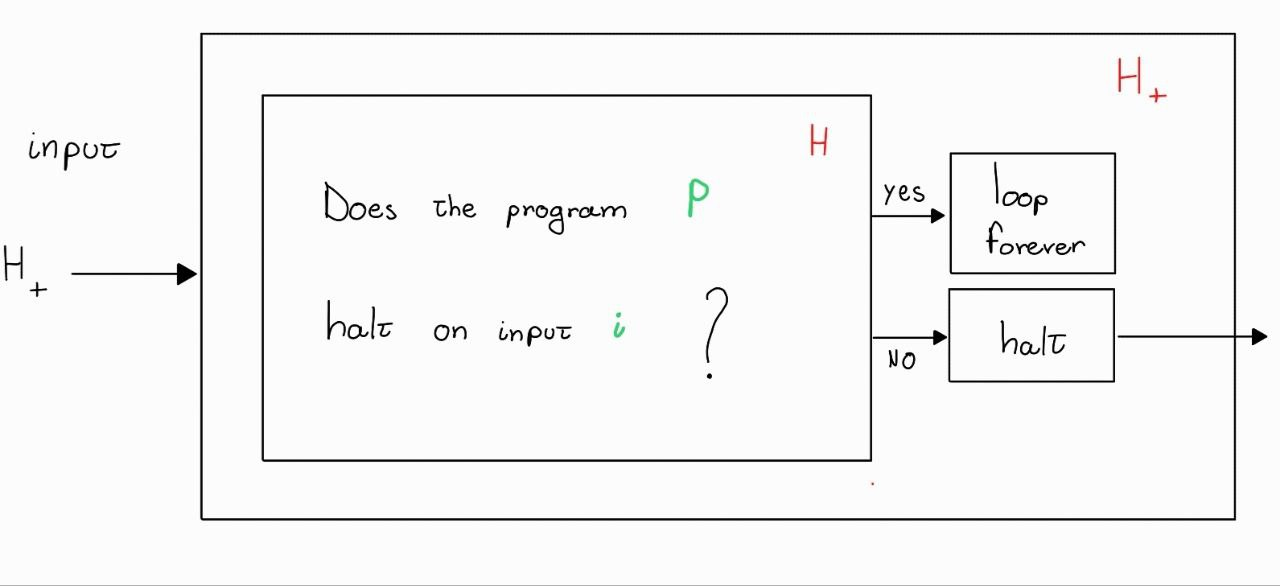
\includegraphics[width=0.5\textwidth]{img/MacchineTuring/halt.png}
        \caption{Rappresentazione grafica della dimostrazione dell'Halting problem}
    \end{figure}
\end{dimostrazione}
\begin{teorema}[\textbf{Halting problem è ricorsivamente enumerabile}]
    Il linguaggio $L_H$ è ricorsivamente enumerabile, ovvero il problema è
    parzialmente decidibile.
\end{teorema}
\begin{dimostrazione}
    Esiste una macchina di Turing $M_A$ che accetta il linguaggio $L_H$, ovvero
    tale che $M_A(M, x) = Y$ se e solo se $M(x) \neq \ \perp$.

    In precedenza abbiamo definito la macchina di Turing universale, la quale
    $U(M, x) = M(x)$, allora:
    \begin{equation}
        M_A(M, x) = \begin{cases}
            Y     & \text{se e solo se} \ U(M, x) = Y \ \lor \ N \\
            \perp & \text{se} \ U(M, x) = \perp
        \end{cases}
    \end{equation}
    Esiste quindi una macchina che accetta il linguaggio $L_H$.
\end{dimostrazione}
\begin{teorema}
    $\overline{L_H}$ non è ricorsivamente enumerabile.
\end{teorema}
\begin{dimostrazione} [\textit{Per assurdo}]
    Assumiamo per assurdo che $\overline{L_H}$ sia ricorsivamente enumerabile.
    Dai teoremi precedenti sappiamo che $L_H$ è ricorsivamente enumerabile, allora
    per quanto definito in precedenza si ha che $L_H$ è ricorsivo, il che è assurdo
    in quanto è stato dimostrato in precedenza che $L_H$ non è ricorsivo.
\end{dimostrazione}
\section{Problemi decidibili}
Vogliamo ora studiare i problemi decidibili classificandoli sulla base dei tempi
di esecuizione, considerando la dimensione dell'input e il caso peggiore. Per fare
questo utilizzeremo il tempo di esecuzione di una macchina di Turing. Questo valore
viene calcolato tramite il numero di passi che la macchina compie.
\begin{definizione}[\textbf{Tempo di calcolo}]
    Definiamo $t_M(x)$ come il tempo di calcolo di una macchina di Turing $M$ su
    input $x$. Non è un caso peggiore ma dipendente dal singolo input specifico.
    Il tempo di calcolo è il numero di passi che esegue $M$ su input $x$ per dare una risposta.
\end{definizione}
Non si usa comunque il numero di passi nella realtà ma si usa la notazione
$\mathcal{O}$-grande, studiando il caso peggiore, ovvero il numero massimo di passi.
\begin{definizione}[\textbf{Complessità temporale}]
    Definiamo $T_M(n)$ come la \textbf{funzione di complessità temporale} come:
    \begin{equation}
        T_M(n) = \max \{t_M(x) \ | \ |x| = n\}
    \end{equation}
\end{definizione}
\begin{definizione}[\textbf{Classe P}]
    Definisco la classe $P$ in base alle macchine di Turing. La classe $P$ è definita come:
    \begin{equation}
        P = \{L \ | \ L \text{ è deciso da una macchina di Turing in tempo polinomiale } \mathcal{O}(p(n))\}
    \end{equation}
\end{definizione}
\begin{definizione}[\textbf{Classe DTIME}]
    Definiamo la classe $DTIME(f(n))$ come la classe dei linguaggi decisi da una
    macchina di Turing entro un tempo $f(n)$:
    \begin{equation}
        DTIME(f(n)) = \{L \subseteq \Sigma^{\ast} \ | \ \exists M \ \text{decide} \ L \ \text{in tempo} \ \mathcal{O}(f(n)) \}
    \end{equation}
    Quindi $DTIME(n)$ rappresenta l'insieme dei problemi di decisione che possono
    essere risolti con un algoritmo che lavora in tempo $\mathcal{O}(n)$. Quindi:
    \begin{equation}
        P = \bigcup_{c \ \in \ \mathbb{N}} DTIME(n^c)
    \end{equation}
    Infatti $P$ è l'unione di tutte le classi DTIME con funzioni polinomiali.
\end{definizione}
\begin{equation}
    DTIME(n) \subseteq DTIME(n^2) \subseteq DTIME(2^{n^c})
\end{equation}
Possiamo anche definire la classe \textbf{EXPTIME} come la classe di linguaggi
decidibili da una macchina di Turing in tempo esponenziale:
\begin{equation}
    EXPTIME =  \bigcup_{c \ \in \ \mathbb{N}} DTIME(2^{n^c})
\end{equation}
Inoltre, si ha che vale la seguente relazione tra le classi $P$ e $EXPTIME$:
\begin{equation}
    P \subseteq EXPTIME
\end{equation}
\begin{teorema}
    Se un problema è nella classe $P$ allora è risolvibile in un tempo efficiente.
\end{teorema}
Devo anche definire la complessità spaziale oltre a quella temporale.
\begin{definizione}[\textbf{Spazio}]
    Definisco lo \textbf{spazio} di calcolo $s_M(x)$ come il numero di celle del
    nastro usate dalla macchina di Turing $M$ con input $x$ durante la computazione.

    Il calcolo non è semplice come per il tempo, avendo anche decrementi. Quindi
    più che “celle usate” studiamo le “celle visitate”.
\end{definizione}
\begin{definizione}[\textbf{Complessità spaziale}]
    Definisco $S_M(n)$ come la \textbf{funzione di complessità spaziale}:
    \begin{equation}
        S_M(n) =  \max\{s_M(x)\ |\  |x| = n\}
    \end{equation}
\end{definizione}
Esiste una relazione tra la complessità spaziale e quella temporale per una macchina
di Turing. Se una computazione dura $n$ passi di tempo, allora posso dire che al
più ho usato $n$ celle di spazio, questo perché è possibile che in alcune
configurazioni la testina non si muove, ma nel caso peggiore si sposta sempre.
Si ha quindi:
\begin{equation}
    S_M(n) \leq T_M(n) + n
\end{equation}
con $+ \ n$ perché sul nastro abbiamo comunque l'input di lunghezza $n$.
\begin{teorema}
    Se il tempo è limitato allora lo spazio è limitato ma non vale l'opposto.
\end{teorema}
\begin{teorema}
    Se ho una macchina di Turing $M$ che lavora in spazio finito e tempo infinito,
    esiste una macchina di Turing $M'$ che fa la stessa cosa di $M$ in tempo
    limitato. Quindi se lo spazio è limitato allora il tempo è limitato.
\end{teorema}
\begin{dimostrazione}
    Infatti la macchina $M'$ può trovarsi in un numero finito di stati $K$ e
    avendo spazio limitato ho un numero limitato $S_M(n)$ di celle in cui si trova
    la testina. Ho anche un numero finito di simboli in alfabeto $\Sigma$ e quindi:
    \begin{equation}
        S_{M'}(n) \leq |k| \cdot |S_M(n)| \cdot |\Sigma|^{|S_M(n)|}
    \end{equation}
    avendo che prima o poi ritorno a stati già visti quindi la macchina se supera
    la quantità appena definita capisce di essere in loop. Quindi
    $|k| \cdot |S_M(n)| \cdot |\Sigma|^{|S_M(n)|}$ è anche un limite temporale
    per la seconda macchina.
\end{dimostrazione}
Quindi data una certa macchina che lavora in un certo spazio $S(n)$ posso costruire
una macchina equivalente che da la stessa risposta in tempo limitato $T(n)$. Si ha
che se ho un problema che si risolve in spazio polinomiale, per la formula appena
scritta avrò tempo esponenziale. Invece, al contrario, tempo polinomiale comporta
spazio polinomiale.
\section{Macchine di Turing non deterministiche}
Una \textbf{macchina di Turing non deterministica} si distingue da quella
deterministica nella funzione di transizione $\delta$. Nella macchina non
deterministica la funzione di transizione associa a ogni stato $q$ e a ogni simbolo
di nastro $X$ un \textit{insieme} di triple:
\begin{equation}
    \delta(q, X) = \{(q_1, Y_1, D_1), (q_2, Y_2, D_2), \dots, (q_k, Y_k, D_k)\}
\end{equation}
A ogni passo una macchina di Turing non deterministica sceglie una delle triple
come mossa, ovviamente lo stato, il simbolo di nastro e la direzione appartengono
alla stessa tripla. Nelle macchine non deterministiche la computazione non è una
sequenza di configurazioni ma un albero di computazione. Da ogni stato posso passare
a uno tra più stati, a seconda della scelta, formando così un albero. Il singolo
passo di computazione non è univocamente definito. Ogni singolo ramo comunque è
equivalente al passo di computazione della macchina di Turing deterministica.
\begin{definizione}[\textbf{Linguaggio accettato}]
    Un linguaggio $L$ è \textbf{accettato} da una macchina di Turing non
    deterministica $N$ se per tutte le stringhe che fanno parte del linguaggio
    esiste almeno una computazione che termina nello stato $Y$, ovvero esiste una
    computazione per cui:
    \begin{equation}
        \forall x \in L \Rightarrow N(x) = Y
    \end{equation}
    Nel caso in cui nessuna delle computazioni termina nello stato $Y$, allora
    l'input non è accettato.
\end{definizione}
\begin{definizione}[\textbf{Linguaggio deciso}]
    Un linguaggio $L$ è \textbf{deciso} da una macchina di Turing non deterministica
    $N$ se, qualora la stringa $x$ appartenga il linguaggio, esiste almeno una
    computazione tale per cui:
    \begin{equation}
        x \in L \to N(x) = Y
    \end{equation}
    altrimenti, se $x$ non appartiene al linguaggio, per tutte le computazioni, si ha che:
    \begin{equation}
        x \not\in L \to N(x) = N
    \end{equation}
    Non devo quindi avere loop in questo caso, tutte devono dare $N$.
\end{definizione}
\begin{teorema}[\textbf{Equivalenza tra macchine di Turing deterministica e non deterministica}]
    Se $M_N$ è una macchina di Turing non deterministica, esiste una macchina di
    Turing deterministica $M_D$ tale che $L(M_N) = L(M_D)$.
\end{teorema}
\begin{dimostrazione}
    La macchina di Turing deterministica $M_D$ simula la macchina di Turing non
    deterministica $M_N$ procede con una visita in ampiezza delle configurazioni
    in modo da evitare di incappare in loop.
\end{dimostrazione}
La macchina di Turing non deterministica $N$ decide il linguaggio $L$ in tempo
$t_N(n)$, ovvero il tempo di calcolo è dato dall'altezza del ramo più lungo.
Come per le macchine deterministiche, definiamo $T_N(n)$ come:
\begin{equation}
    T_N(n) = \max \{t_N(x) \ | \ |x| = n\}
\end{equation}
Data una macchina di Turing non deterministica $N$ che decide $L$ in tempo $T_N(n)$
esiste una macchina di Turing deterministica $M$ che decide $L$ in tempo
$2^{\mathcal{O}(T_N(n))}$. Questa complessità deriva dal fatto che se ogni nodo
dell'albero ha al massimo $b$ figli, allora l'albero di computazione ha al massimo
$b^{T_N(n)}$ foglie. Il numero interno di nodi è al massimo $b^{T_N(n)} - 1$ e
quindi il numero totale di nodi è $< 2 \cdot b^{T_N(n)}$. Inoltre, un cammino
dalla radice alla foglia è $\mathcal{O}(T_N(n))$. Il tempo di esecuzione della
macchina $M$ è $\mathcal{O}(T(n) \cdot b^{T(n)})$ che può essere visto come
$2^{\mathcal{O}(T_N(n))}$.
\begin{definizione}[\textbf{Classe NTIME}]
    Definiamo una funzione di tempo per una macchina di Turing non deterministica come:
    \begin{equation}
        NTIME = \{L \ | \ L \ \text{è deciso da una macchina di Turing non deterministica in tempo } \mathcal{O}(f(n))\}
    \end{equation}
\end{definizione}
Quest'ultima definizione ci permette di definire la classe di \textbf{problemi NP}
come l'insieme dei linguaggi $L$ che sono decisi in tempo polinomiale da una macchina
di Turing non deterministica:
\begin{equation}
    NP = \bigcup_{c > 0} NTIME(n^c)
\end{equation}
\begin{osservazione}
    Sia $P$ l'insieme dei \textbf{problemi decidibili in tempo polinomiale} da una
    macchina di Turing deterministica, e $NP$ l'insieme dei \textbf{problemi decidibili in tempo polinomiale}
    da una macchina di Turing non deterministica. Sappiamo che è vero che $P \subset NP$
    ma non è ancora dimostrato che $NP \subset P$.
\end{osservazione}
Possiamo quindi affermare che:
\begin{equation}
    P \subseteq NP \subseteq EXPTIME
\end{equation}
$NP$ rappresenta una classe di linguaggi che sono verificabili in tempo polinomiale
da una macchina di Turing non deterministica. Verificare un linguaggio significa
che per ogni parola $w \in L$ si ha una stringa $c$ detta \textbf{certificato} che
possiamo usare per verificare che effettivamente $w \in L$.
\begin{definizione}
    Un \textbf{verificatore} di un linguaggio $L$ è una macchina di Turing
    deterministica $V$ tale per cui:
    \begin{equation}
        L = \{w : V \ \text{accetta} \ \langle w, c \rangle \ \text{per qualunque stringa} \ c\}
    \end{equation}
    Questa macchina accetta le stringhe appartenenti al linguaggio eseguendo le
    istruzioni specificate dal certificato $c$.
\end{definizione}
Se $V$ richiede tempo polinomiale rispetto $w$ a per accettare/rifiutare, allora
$V$ è un verificatore in tempo polinomiale per $w$. Se esiste un verificatore in
tempo polinomiale per $L$, allora $L$ è verificabile in tempo polinomiale.

Dato che $V$ deve eseguire in tempo polinomiale rispetto a $w$, ne segue che $c$,
il certificato, deve essere di lunghezza polinomiale rispetto a $w$, altrimenti
non avremmo il tempo di leggere tutto $c$.

Supponiamo di avere una macchina di Turing non deterministica $M$ che lavora in
tempo polinomiale, costruiamo un verificatore $V$ che lavora in tempo polinomiale
per lo stesso linguaggio deciso da $M$. Se su input $w$ la macchina $M$ accetta,
significa che esiste una computazione accettante $C_1, \dots, C_k$ di lunghezza
polinomiale rispetto a $w$. Per ogni passaggio da $C_i$ a $C_{i + 1}$ è stata applicata
una transizione definita dalla funzione di transizione di $M$.

Usiamo come certificato $c$ la sequenza di transizioni applicate lungo tutta la
computazione, le quali sono in numero polinomiale. Queste transizioni ci identificano
una specifica computazione della macchina di Turing non deterministica $M$.
Il verificatore deve solo simulare quella computazione, senza fare scelte non
deterministiche, dato che le transizioni da fare sono tutte in $c$ e verificare
che la computazione accetti.

Abbiamo mostrato che per ogni linguaggio accettato da una macchina di Turing non
deterministica che lavora in tempo polinomiale possiamo costruire un verificatore
polinomiale per lo stesso linguaggio. Dobbiamo mostrare anche l'inclusione in senso
inverso. Sfruttiamo il fatto che possiamo usare una macchina di Turing non
deterministica per scrivere un certificato sul nastro e, se esiste un certificato
che ci permette di accettare, questo sarà presente in una computazione.

Sia $V$ un verificatore in tempo polinomiale per $L$. Assumiamo $V$ esegua in
tempo $n^k$. Costruiamo una macchina di Turing non deterministica che su input $w$ fa due cose:
\begin{itemize}
    \item Genera in modo non deterministico un certificato $c$ di lunghezza al più $n^k$.
    \item Simula $V$ su input $\langle w, c \rangle$ e accetta se $V$ accetta,
          mentre rifiuta se $V$ rifiuta.
\end{itemize}
Abbiamo mostrato che per ogni linguaggio per il quale esiste un verificatore
polinomiale possiamo costruire una macchina di Turing non deterministica che decide
lo stesso linguaggio in tempo polinomiale. Quindi le due definizioni di $NP$ sono equivalenti.

Definiamo ora altre classi di problemi:
\begin{itemize}
    \item Linguaggi di cui posso decidere la \textbf{non appartenenza} in tempo polinomiale:
          \begin{equation}
              coP = \{L \ | \ \overline{L} \in P\}
          \end{equation}
    \item Linguaggi che \textbf{non sono decidibili} in tempo polinomiale: $\overline{P}$
    \item Linguaggi di cui posso decidere la \textbf{non appartenenza} in tempo
          polinomiale da una macchina di Turing non deterministica:
          \begin{equation}
              coNP = \{L \ | \ \overline{L} \in NP\}
          \end{equation}
\end{itemize}
\begin{nota}
    \begin{equation}
        \overline{P} \neq coP
    \end{equation}
    \begin{equation}
        P \subseteq NP \ \land \ P \subseteq coNP \ \text{quindi} \ P \subseteq NP \cap coNP
    \end{equation}
\end{nota}
\begin{teorema}
    \begin{equation}
        P = coP
    \end{equation}
\end{teorema}
\begin{dimostrazione}
    Se un linguaggio $L \in P$, allora esiste una macchina di Turing deterministica
    che decide $L$ in tempo polinomiale:
    \begin{equation}
        \forall x \in \Sigma^{\ast} = \begin{cases}
            x \in L \Rightarrow M(x) = Y \\
            x \not\in L \Rightarrow M(x) = N
        \end{cases}
    \end{equation}
    Posso inoltre creare una macchina $M'$ che decide $\overline{L}$ in tempo polinomiale:
    \begin{equation}
        \forall x \in \Sigma^{\ast} = \begin{cases}
            x \in \overline{L} \Rightarrow M'(x) = Y \\
            x \not\in \overline{L} \Rightarrow M'(x) = N
        \end{cases}
    \end{equation}
    per ottenere questa macchina è sufficiente modificare gli stati di accettazione
    e rifiuto della macchina $M$.
\end{dimostrazione}
La dimostrazione precedente non può essere utilizzata per dimostrare che $NP = coNP$
dato che, nel caso di macchine non deterministiche è sufficiente che esista un singolo
ramo di computazione che termina in uno stato di accettazione. Invertendo l'output di questa
macchina si ottiene una macchina che non decide $\bar{L}$ dato che sarebbero necessaire
tutte computazioni che terminano in uno stato accettante.
\section{Riduzioni polinomiali}
Le \textbf{riduzioni polinomiali} tra problemi sono delle procedure che per ogni
istanza del problema $A$ la trasformano in un'istanza per un problema diverso $B$.
Quindi un'istanza di $A$, $I_A$, ha due risposte, $Y$ o $N$, ma posso passare tramite
una determinata funzione:
\begin{equation}
    f: I_A \to I_B
\end{equation}
avendo poi $I_B$ tale che $B$ avrà risposte, uguali a quelle di $A$, $Y$ o $N$.
In altre parole, si cerca una funzione $f$ che mi permette di convertire le
istanze del mio problema di partenza in istanze di un problema che so risolvere.
\begin{definizione}[\textbf{Riduzione polinomiale}]
    La \textbf{riducibilità polinomiale} tra problemi è definita come:
    \begin{equation}
        f: \Sigma^{\ast} \to \Sigma^{\ast}
    \end{equation}
    la quale deve essere calcolabile in tempo polinomiale da una macchina di Turing
    deterministica, tale che:
    \begin{equation}
        \forall x \in \Sigma^{\ast}, \ x \in L_A \ \text{se e solo se} \ f(x) \in L_B
    \end{equation}
    Indichiamo l'operazione di riduzione polinomiale come:
    \begin{equation}
        L_A \leq_P L_B
    \end{equation}
\end{definizione}
\begin{osservazione}
    Si utilizza il simbolo minore uguale, per indicare una relazione d'ordine
    nella complessità dei problemi.
\end{osservazione}
\begin{teorema}
    Dato un linguaggio $L_A$ riducibile polinomialmente a $L_B$ ($L_A \leq_P L_B$),
    si ha che se $L_B \in P$ allora sicuramente anche $L_A \in P$.
\end{teorema}
\begin{dimostrazione}
    Infatti e esiste un algoritmo polinomiale per $L_B$ allora, avendo una
    trasformazione polinomiale ho che $f(x) + L_B$ è ancora polinomiale.
\end{dimostrazione}
\begin{teorema}
    La riduzione polinomiale gode della proprietà di transitività, ovvero:
    \begin{equation}
        L_A \ \leq_P \ L_B \ \land \ L_B \ \leq_P \ L_C \ \text{allora} \ L_A \ \leq_P \ L_C
    \end{equation}
    Posso ottenere questa riduzione applicando la composizione di funzioni.
\end{teorema}
\begin{definizione}[\textbf{NP-hard}]
    Un linguaggio $L$ è $\textbf{NP}\_\textbf{hard}$ se vale che:
    \begin{equation}
        \forall L' \in NP \ \text{si ha} \ L' \leq_P L
    \end{equation}
\end{definizione}
\begin{definizione}[\textbf{NP-completo}]
    Un linguaggio $L$ si dice $\textbf{NP}\_\textbf{completo}$ se valgono i
    seguenti punti:
    \begin{itemize}
        \item $L \in NP$
        \item $L \in NP\_hard$
    \end{itemize}
\end{definizione}
\begin{teorema}
    Se $L_A \leq_P L_B$ e $L_A \in NP\_hard$ allora so che anche $L_B \in NP\_hard$.
\end{teorema}
\begin{dimostrazione}
    Se $L_A \leq_P L_B$ per la definizione di $NP\_hard$ so che esistono n linguaggi
    che sono riducibili polinomialmente a $L_A$. Utilizzando la proprietà transitiva
    posso affermare che $L_B$ è $NP\_hard$.
\end{dimostrazione}
\begin{teorema}[\textbf{Teorema Cook-Levin}]
    Il problema di soddisfacibilità SAT è $NP\_completo$. Questo problema prende
    in input una formula booleana $\phi$ in forma normale congiunta (CNF), ovvero
    che ha una congiunzione ($\land$) come legame tra le clausole. Una clausola
    è un $\lor$ di letterali, ovvero di variabili booleane $x_i$ o $\overline{x_i}$.
    In output ho se la forma sia soddisfacibile o meno.
\end{teorema}
\begin{figure}[!ht]
    \centering
    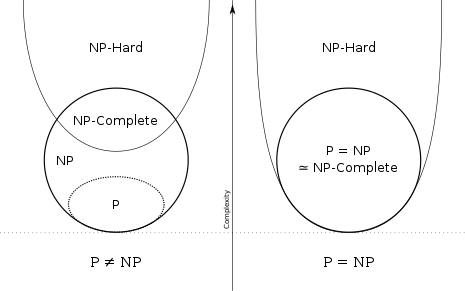
\includegraphics[width=0.5\textwidth]{img/MacchineTuring/classificazioneProblemi.png}
    \caption{Classificazione dei problemi.}
\end{figure}
% https://en.wikipedia.org/wiki/Succinct_data_structure
\chapter{Strutture dati succinte}
Le \textbf{strutture dati succinte} sono una classe di strutture dati che forniscono un compromesso tra l’efficienza dell’accesso ai dati e la quantità di spazio utilizzato per memorizzare i dati. Queste strutture cercano di minimizzare l’uso dello spazio di memoria, mantenendo nel contempo un accesso efficiente ai dati.

Le strutture dati succinte sono un tipo di struttura dati che utilizza una quantità di spazio “vicina” al limite inferiore teorico dell’informazione, ma che, a differenza di altre rappresentazioni compresse, consente ancora operazioni di interrogazione efficienti.

A differenza degli algoritmi generali di compressione dei dati senza perdita, le strutture dati succinte mantengono la capacità di utilizzarle sul posto, senza prima decomprimerle.

Supponiamo che $\mathcal{Z}$ sia il numero ottimale teorico di bit necessari per memorizzare alcuni dati. Una rappresentazione di questi dati viene chiamata:
\begin{itemize}
    \item \textbf{Implicita} se richiede $\mathcal{Z} + \mathcal{O}(1)$ bit di spazio. (es. $\mathcal{Z} + 14$ bit) 
    \item \textbf{Succinta} se richiede $\mathcal{Z} + o(\mathcal{Z})$ bit di spazio. (es. $\mathcal{Z} + \log \mathcal{Z}$ oppure $\mathcal{Z} + \sqrt{\mathcal{Z}}$ bit)
    \item \textbf{Compatta} se richiede $\mathcal{O}(\mathcal{Z})$ bit di spazio. (es. $5\mathcal{Z}$ bit)
\end{itemize}
\begin{nota}
    $o(\mathcal{Z})$ si riferisce al concetto matematico di \textit{o-piccolo}, ovvero:
    \begin{equation}
        \lim_{x \to x_0} \frac{f(x)}{g(x)} = 0 \Rightarrow f(x) = o_{x_0} (g(x)) \ \text{con} \ x_0 = + \infty
    \end{equation}
\end{nota}
\section{Bitvector}
Le strutture dati vengono rappresentate per mezzo di \textbf{bitvector}.
\begin{definizione}
    Si definisce un \textbf{bitvector} $B$ come un array di lunghezza $n$, popolato da elementi binari. Formalmente si ha:
    \begin{equation}
        B[i] \in \{0, 1\}, \ \forall i \ \text{tale che} \ 1 \leq i \leq n
    \end{equation}
    In alternativa all'alfabeto binario è possibile utilizzare i valori booleani vero e falso.
\end{definizione}

Su questa struttura è possibile effettuare due operazioni:
\begin{itemize}
    \item \textbf{rank}: restituisce il numero di elementi uguali a $q$ che sono presenti nella struttura dati fino a $x$.
    \begin{equation}
        rank_q(x) = \sum_{k = 1}^{k \leq i} B[k], \ \forall i \ \text{tale che} \ 1 \leq i \leq n \ \land \ B[k] = q
    \end{equation}
    \item \textbf{select}: restituisce la posizione della $x$-esima occorrenza di $q$.
    \begin{equation}
        select_q(x) = \min{\{k \in [0, \dots, n): \ rank_q(k) = x\}}
    \end{equation}
\end{itemize}
\begin{nota}
    \begin{equation}
        rank_q(select_q(i)) = i
    \end{equation}
\end{nota}

È possibile ottenere una struttura dati succinta, usando $o(n)$ bit aggiuntivi, che permetta di effettuare le operazioni di \textit{rank} e \textit{select} in tempo costante $\mathcal{O}(1)$.
\subsection{Funzione rank}
Vediamo ora come è possibile rendere il tempo di esecuzione dell'operazione di rank costante. 

Memorizzare tutti i valori di $rank(i)$ necessiterebbe di $O(n \log n)$ bit il che non lo rende un o-piccolo di $n$. Memorizzo quindi ogni $l-$esimo valore $rank(i)$, a questo punto, a query time scorriamo i restanti $l-1$ bit.

Questi valori vengono salvati in un vettore \textit{first} $F[0 \dots n / l]$, dove $/$ indica la divisione intera, tale che:
\begin{itemize}
    \item $F[0] = 0$
    \item $F[i / l] = rank(i)$ se $i \mod l = 0$
\end{itemize}

Se $l = \left(\left\lceil \frac{\log n}{2} \right\rceil \right)^2$ si ha un ordine di $\frac{n}{\log n}$ bit per l'array $F$. Con questa prima operazione è possibile eseguire una rank come:
\begin{equation}
    rank(i) = F[i/l] + C(B[l \cdot (i / l) + 1 \dots i])
\end{equation}
con $C(B')$ che rappresenta una funzione che conta i simboli $\sigma = 1$ in $B'$. Questa soluzione mi porta a una rank eseguita in tempo $\mathcal{O}( \log^2 n )$.

Possiamo ridurre ulteriormente questo tempo tenendo in memoria più informazioni. 

In ogni blocco di lunghezza $l$ indotto da $F$ memorizziamo ogni $k$ posizioni il numero di simboli $\sigma = 1$ a partire dall'inizio del blocco, escludendo la posizione iniziale in cui il valore di rank è già in $F$. Otteniamo un vettore \textit{second} $S[0 \dots l /k]$ con:
\begin{equation}
    S[i/k] = rank_{B[l \cdot (i / l) + 1 \dots i]} (i - l \cdot (i / l) + 1)
\end{equation} quando $i \mod k = 0$.

Questa soluzione richiede $\mathcal{O}((\frac{n}{k}) \log l)$ bit aggiuntivi. In particolare, scegliendo $k = \left\lceil \frac{\log n}{2} \right\rceil$ si ottiene uno spazio di $\mathcal{O}(\frac{n \log \log n}{\log n})$ bit. Introducendo quest secondo vettore è possibile eseguire una rank come:
\begin{equation}
    rank(i) = F[i/l] + S[i /k] + C(B[k \cdot (i / k) + 1 \dots i])
\end{equation}
Questa soluzione mi porta a una rank eseguita in tempo $\mathcal{O}(\log n )$.

Per ottenere una rank in tempo costante si utilizza la tecnica \textbf{Four Russians technique}. Questa tecnica consiste nel salvare una look-up table third $T$, di dimensioni $2^{k - 1} \times k - 1$. $T$ salva i valori di $rank(i')$ per tutte le posizioni $k - 1$ in tutte le possibili configurazioni indotte dai blocchi definiti per $S$. $T$ richiede uno spazio pari a $\mathcal{O}(\sqrt{n} \log n \log \log n)$ bit.

Si definisce $c_i = B[k \cdot (i / k) + 1 \dots k \cdot (i / k + 1) - 1]$ come il bitvector di lunghezza $k - 1$ che copre il $(k + 1)-$esimo blocco. Usando l'operatore modulo posso sapere la posizione relativa di $i$ in questo bitvector e accedere alla lookup table dove la riga è indicizzata da $c_i$ e la colonna dalla posizione relativa in tempo $\mathcal{O}(1)$.
\begin{equation}
    rank(B) = \begin{cases}
        F[i/l] & \text{se} \ i \mod l = 0 \\
        F[i/l] + S[i/k] & \text{se} \ i \mod l \neq 0 \land i \mod k = 0 \\
        F[i/l] + S[i/k] + T[c_i][(i \mod k) - 1]& \text{se} \ i \mod l \neq 0 \land i \mod k \neq 0 \\
    \end{cases}
\end{equation}

In questo modo, memorizzando un $o(n)$ bit in più posso eseguire l'operazione di rank in tempo costante. La costruzione della struttura avviene però in tempo lineare.
\begin{esempio}
    Vediamo un esempio di come può essere implementata la funzione rank in modo da effettuare accesso in tempo costante. Scegliamo i valori di $l = 9$ e $k = 3$ e otteniamo:
    \begin{figure}[!ht]
        \centering
        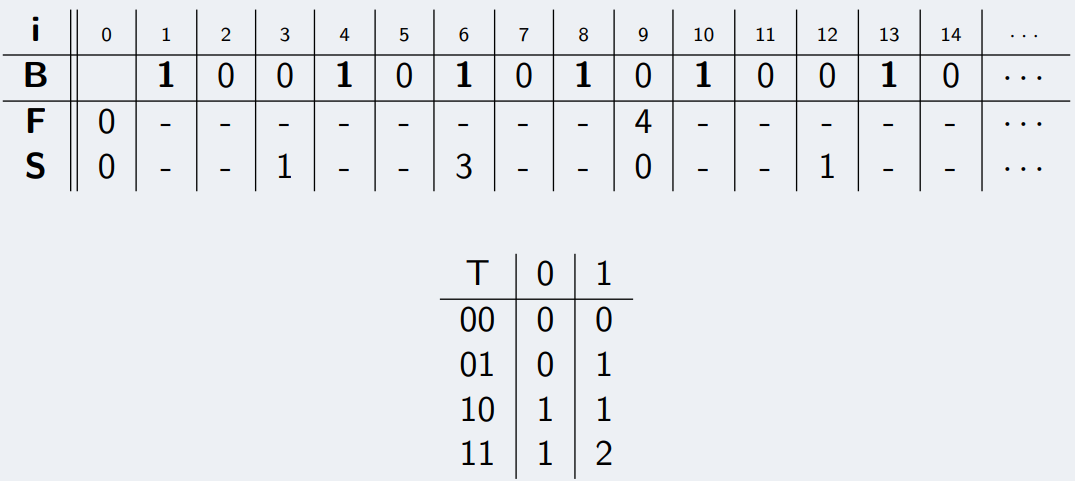
\includegraphics[width=0.5\textwidth]{img/Strutture Dati/rank.png}
        \caption{Esempio di implementazione della funzine rank}
    \end{figure}
\end{esempio}
\begin{osservazione}
    Si può dimostrare che, con un procedimento abbastanza analogo a quello visto per la funzione di rank, è possibile costruire una struttura che necessita di $o(n)$ bit aggiuntivi e che permette di effettuare l'operazione di select in tempo costante.
\end{osservazione}
\section{Level Order Unary Degree Sequence}
Consideriamo in memoria la rappresentazione di un albero etichettato con $n$ nodi. Una rappresentazione a pointer richiede $\mathcal{O}(n \log n)$ spazio. 

Analizziamo ora una rappresentazione basata sulla visita in left-to-rigth level-order di un albero, ovvero una visita in ampiezza. In questa rappresentazione si considera un nodo detto \textbf{super-root}. A questo punto si memorizza la sequenza $D$ dei gradi dei nodi. Questa sequenza viene memorizzata utilizzando un prefix code binario, dove per ogni nodo visitato si aggiunge a un bitvector $B$ i simboli della sequenza $1^d0$, con $d$ che rappresenta il grado del nodo. La super-root viene aggiunta in modo che il numero di 1 presenti nella sequenza sia uguale al numero di nodi dell'albero.

In questo modo si arriva a ottenere un bitvector di lunghezza $2n + 1$ dove si ha un simbolo 1 associato a ogni nodo dell'albero. Con questa rappresentazione posso indicare il nodo $m$ con l'indice relativo del corrispondente bit 1.

Utilizzando le operazioni rank e select definite per il bitvector, è possibile implementare un set di operazioni per interrogare questa rappresentazione dell'albero.
\begin{itemize}
    \item $is\_leaf(v) = T$ se e solo se $select_0(v) = select_0(v + 1) - 1$ in quanto per costruzione una foglia aggiunge solo uno 0 al bitvector $B$, quindi con $select_0(v)$ troviamo la posizione dello 0 posto in $B$ dal nodo antecedente a $v$ nella visita (quello antecedente perché abbiamo il 10 della super-root) e con $select_0(v + 1)$ la posizione dello 0 relativo a $v$. Se sono in due posizioni adiacenti significa che $v$ ha aggiunto solo uno $0$ e quindi è una foglia.
    \item $first\_child(v) = rank_1(select_0(rank_1(select_1(v)))+1) = rank_1(select_0(v)+1)$:
    \begin{itemize}
        \item $k = select_0(v) + 1$ restituisce la posizione $k$ su $B$ del primo "figlio" di $v$. In altri termini il $v$-esimo 0 mi dice che ho finito di "visitare" la sotto-sequenza di bitvector costruita per il nodo $v - 1$ e al bit successivo inizia la sequenza del bitvector per $v$.
        \item $m = rank_1(k)$ restituisce il numero di nodo dell'albero in posizione $k$ di $B$, quindi la label del primo "figlio" di $v$.
        \item Imponiamo che $first\_child(v) = - 1$ se $is\_leaf (v) = T$
    \end{itemize}
    \item $last\_child(v) = rank_1(select_0(rank_1(select_1(v))+1)-1) = rank_1(select_0(v+1)-1)$:
    \begin{itemize}
        \item $k = select_0(v + 1)$ restituisce la posizione $k$ su $B$ dello $0$ inserito in visita level-order del nodo con label $v$. In altri termini, il (v + 1)-esimo 0 mi dice che ho finito di "visitare" la sotto-sequenza di bitvector costruita per il nodo $v$.
        \item $w = k - 1$ restituisce l'indice dell'ultimo 1 inserito in visita level-order del nodo con label j, quindi l'indice su B dell'ultimo "figlio" di c. In altri termini, con la precedente operazione si raggiunge lo 0 di $1^d 0$ e col -1 l'ultimo 1 di $1^d$
        \item $m = rank_1(w)$ restituisce il numero di nodo dell'albero in posizione $w$ di B, quindi la label dell'ultimo "figlio" di v.
        \item Imponiamo che $last\_child(v) = -1$ se $is\_leaf (v) = T$
    \end{itemize}
    \item $parent(v) = rank_1(select_1(rank_0(select_1(v)))) = rank_0(select_1(v))$:
    \begin{itemize}
        \item $i = select_1(v)$ restituisce la posizione $i$ del nodo $v$ nel bitvector $B$ (identificando in quale $1^d 0$ è stato aggiunto).
        \item $j = rank_0(i)$ restituisce il numero di sequenze che sono state aggiunte al bitvector $B$ fino a quella relativa al "genitore" del nodo in posizione $i$. Il numero di tali sequenza è l'indice del nodo "genitore" per definizione di vista level order e conseguente etichettatura dei nodi.
        \item Imponiamo che $parent(v) = -1$ se $v = 1$ (non considero la super-root)
    \end{itemize}
    \item $degree(v) = last\_child(v) - first\_child(v) + 1$, imponiamo $degree(v) = 0$ se $last\_child(v) = first\_child(v) = -1$
    \item $nth\_child(v, nth) = rank_1(select_1(first\_child(v)) + nth - 1)$, imponiamo $nth\_child(v, nth) = -1$ se $degree(v) < nth$
\end{itemize}
\begin{esempio}
    Costruzione di un e Level Order Unary Degree Sequence:
    \begin{figure}[!ht]
        \centering
        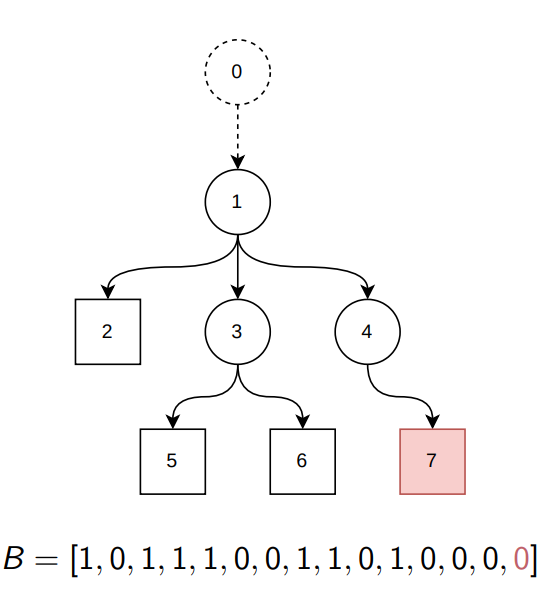
\includegraphics[width=0.6\textwidth]{img/Strutture Dati/LOUDS.png}
        \caption{Esempio di costruzione di un e Level Order Unary Degree Sequence}
    \end{figure}
\end{esempio}
\section{Wavelet Tree}
Abbiamo visto come rank e select possono essere usati per interrogare un bitvector, che ha un alfabeto fisso di grandezza 2. Siamo ora interessati a generalizzare tali query ad un alfabeto di grandezza arbitraria. Per praticità assumiamo $\Sigma = [1 \dots s]$ ordinato: $\Sigma[i] \prec \Sigma[j] \iff i < j \dots$.

Dato un generico alfabeto $\Sigma$ e una sequenza $T[1\dots n] \in \Sigma$:
\begin{itemize}
    \item $rank_{\sigma,T} (i)$ conta tutte le occorrenze del simbolo $\sigma \in \Sigma$ fino all'indice $i$ in $T$, $i \leq | T |$
    \item $select_{\sigma,T} (i)$ ritorna la posizione dell'i-esima occorrenza del simbolo $\sigma \in \Sigma$ in $T$, $i \leq | T |$
\end{itemize}
\begin{equation}
    rank_{\sigma,T} (select_{\sigma,T} (i)) = i, \ \forall \sigma \in \Sigma \land \forall i = 1 \dots n
\end{equation}


Una rappresentazione "naïve" consiste nel considerare come rappresentazione di $T$ un insieme di $| \Sigma | = s$ stringhe binarie $B_\sigma[1\dots n], \ \forall \sigma \in \Sigma$ si ha che:
\begin{equation}
    B_\sigma[i] = 1 \iff T[i] = \sigma \ \text{e} \ B_\sigma[i] = 0  \iff T[i] \neq \sigma
\end{equation}

Se per ogni bitvector $B_\sigma$ abbiamo calcolato la struttura a supporto vista precedentemente si ha $rank_{\sigma,T} (i)$ in tempo costante $\mathcal{O}(1)$ e uno spazio pari a $s \cdot (n + o(n))$ bit aggiuntivi.

Possiamo ottenere una rappresentazione più efficiente in memoria senza sacrificare troppo i tempi di query. Per realizzare questa rappresentazione consideriamo un \textbf{albero binario perfettamente bilanciato} dove ogni nodo corrisponde ad un sottoinsieme di $\Sigma$. 

I due figli di ogni nodo partizionano il corrispondente sottoinsieme di $\Sigma$ in due. A ogni nodo $v$ corrisponde una sequenza chiamata $R_v$ (sotto-sequenza dell'input $T$), la quale è sotto-sequenza di quella con cui è etichettato il nodo genitore di $v$. Alla root corrisponde la sequenza $R_v = T$.

A ogni nodo $v$ si associa un bitvector, denotato con $B_v$, che indica a quale dei due figli del nodo $v$ ogni simbolo della sotto-sequenza $R_v$ appartiene. Ad esempio con $1 \leq j \leq |R_v|$ se $B_v [j] = 0$ allora il carattere associato $R_v [j]$ appartiene alla sotto-sequenza rappresentata dal figlio di sinistra, mentre se $B_v [j] = 1$ allora il carattere associato a $R_v [j]$ appartiene alla sotto-sequenza rappresentata dal figlio di destra.

Le foglie dell'albero sono \textit{virtualmente} etichettate con i singoli caratteri dell'alfabeto. In realtà ci basta la funzione $rank_1$ eseguita sui bitvector che etichettano i genitori delle foglie per recuperare l'informazione.

Vediamo ora come realizzare le operazioni su questa struttura dati:
\begin{itemize}
    \item \textbf{rank}: si inizia il calcolo nel nodo root e si determina a quale dei due figli appartiene $\sigma$, tramite l'ordinamento dell'alfabeto. Nella radice se $B_v [j] = 0$ allora $R_v [j] = \sum [\lceil \frac{s}{2} \rceil] \lor R_v [j] \prec \Sigma[\lceil \frac{s}{2} \rceil]$, altrimenti se $B_v[j] = 1$ allora il carattere che si cerca è nella seconda metà dell'alfabeto. 

    A questo punto si prosegue nel seguente modo:
    \begin{itemize}
        \item se $\sigma = \Sigma [ \lceil \frac{s}{2} \rceil] \lor \sigma \prec \Sigma [\lceil \frac{s}{2}\rceil]$ allora si prosegue verso il "figlio" di sinistra, aggiornando $i$ con $i = rank_{0,B_v}(i)$
        \item Altrimenti usiamo il "figlio" di destra, aggiornando $i$ con $i = rank_{1,B_v}(i)$.
    \end{itemize}
    Nel nuovo $v$ si procede nello stesso modo, considerando che ora $\Sigma = \Sigma [1 \dots \lceil \frac{s}{2} \rceil]$ se si è andati a sinistra e $\Sigma = \Sigma [\lceil \frac{s}{2} \rceil + 1 \dots s]$ se a destra.
    
    Si prosegue fino ad una foglia e $rank_{\sigma,T} (i) = i'$, dove $i'$ è l'ultimo valore di i che si ottiene nei vari step.
    
    L'albero ha altezza $\lceil \log s\rceil$ quindi $rank_{\sigma,T} (i)$ può essere calcolato in $\mathcal{O}(\log s)$.

    \item \textbf{random access}: in questo caso la scelta del figlio dipende unicamente da $B_v [i]$:
    \begin{itemize}
        \item Se $B_v [i] = 0$ proseguo verso il "figlio" di sinistra, con $i = rank_{0,B_v}(i)$
        \item Se $B_v [i] = 1$ proseguo verso il "figlio" di destra, con $i = rank_{1,B_v}(i)$
    \end{itemize}
    
    $T[i]$ è il simbolo che etichetta la foglia raggiunta alla fine della visita dato che il wavelet tree di una sequenza $T$ garantisce random access alla sequenza stessa possiamo sostituirla col suo wavelet tree.

    L'albero ha altezza $\lceil\log s \rceil$ quindi $access_{\sigma,T} (i)$ può essere calcolato in $\mathcal{O}(\log s)$.

    \item \textbf{select}: analogamente ai bitvector si può dimostrare che anche $select_{\sigma,T}(i)$ può essere calcolato in $\mathcal{O}(\log s)$
\end{itemize}
Vediamo ora come costruire un wavelet tree livello per livello a partire dalla root:
\begin{enumerate}
    \item Si etichetta la root con $R_v = T$ e un bitvector $B_v$ tale che $\forall 1 \leq i \leq |T|$: 
    \begin{itemize}
        \item $B_v[i] = 0 \iff T[i] = \Sigma[\lceil \frac{s}{2} \rceil] \lor T[i] \prec \Sigma[\lceil \frac{s}{2} \rceil]$
        \item $B_v[i] = 1$ altrimenti.
    \end{itemize}
    \item Si estrae la sotto-sequenza $T'$ corrispondente ai valori 0 di $B_v$ e la si usa per etichettare il "figlio" di sinistra $v_1$ (che è relativo all'alfabeto $\Sigma = \Sigma[1 \dots \lceil \frac{s}{2} \rceil]$) mentre quella corrispondente ai valori 1 la si usa per etichettare il "figlio" di destra $v_2$ (che è relativo all'alfabeto $\Sigma = \Sigma[\lceil \frac{s}{2} \rceil + 1 \dots s]$) per entrambe
    \item Posso quindi cancellare $T$ e costruire i bitvector $B_{v1}$ e $B_{v2}$, con le rispettive strutture per la funzione rank e continuare ricorsivamente fino al raggiungimento delle foglie (quando si raggiungono alfabeti di cardinalità 1).
\end{enumerate}
Il processo di costruzione di un wavelet tree richiede un tempo pari a $\mathcal{O}(n \log s)$.

In ogni momento della costruzione del wavelet tree abbiamo un bound in spazio pari a $3n \log s + \mathcal{O}(s \log n)$, dato da:
\begin{itemize}
    \item 3 sottosequenze di $T$, quella del "genitore" e quelle dei due "figli".
    \item Tutti i bitvector finora computati che formano il wavelet tree.
    \item I puntatori che memorizzano la struttura ad albero.
\end{itemize}

Un ulteriore miglioramento in spazio si può ottenere concatenando tutti i bitvector in un unico bitvector con una sola struttura a supporto della funzione rank. In tal caso la struttura ad albero si può inferire dai partizionamenti dell'alfabeto e dai bitvector. Questa variante è chiamata \textbf{levelwise wavelet tree}.

Un wavelet tree per una sequenza lunga $n$ costruita su alfabeto di cardinalità $s$ occupa, avendo $\mathcal{O}(s \log n)$ per la topologia dell'albero:
\begin{equation}
    n \log s + o(n \log s) + \mathcal{O}(s \log n) \ bit
\end{equation}

Mentre, un levelwise wavelet tree richiede:
\begin{equation}
    n \log s + o(n \log s) \ bit
\end{equation}
\begin{esempio}
    Costruzione di un wavelet tree:
    \begin{figure}[!ht]
        \centering
        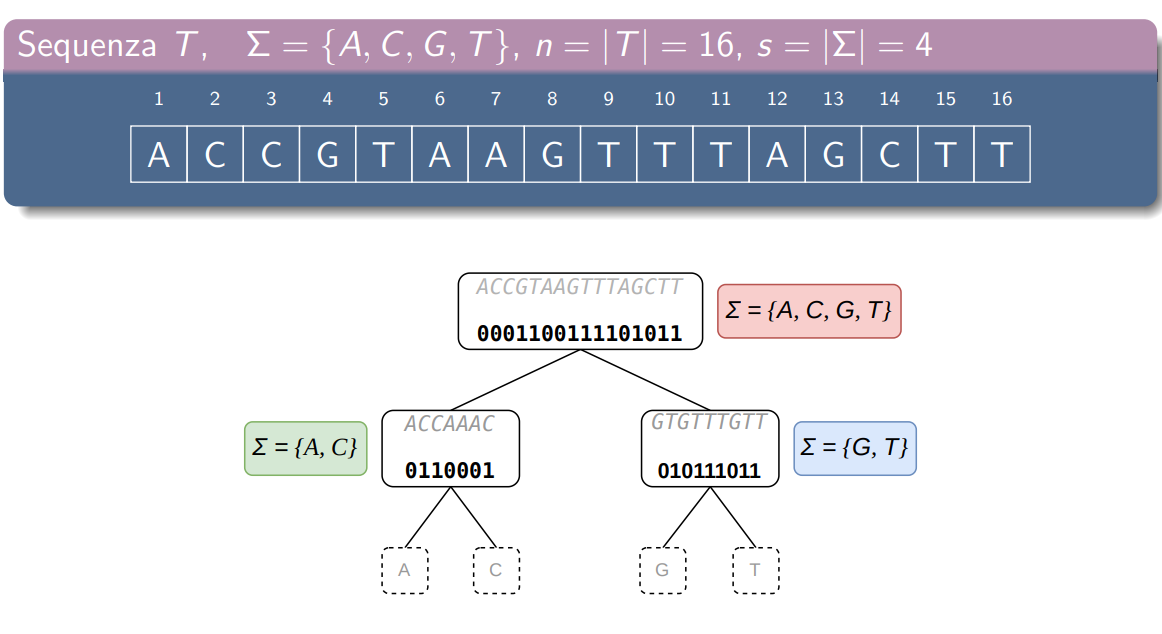
\includegraphics[width=0.7\textwidth]{img/Strutture Dati/wavelet tree.png}
        \caption{Esempio di costruzione di un wavelet tree su una sequenza semplice}
    \end{figure}
\end{esempio}
\section{Altre strutture dati succinte}
\begin{itemize}
    \item \textbf{Parentesi bilanciate}: si costruisce a partire dalla DFS dell'albero (preorder):
    \begin{itemize}
        \item "(" quando si raggiunge un nodo per la prima volta.
        \item ")" quando si è terminata la visita del sottoalbero.
    \end{itemize}
    \item Strutture dati succinte che supportano le \textbf{range minimum queries}.
    \item \textbf{Wavelet matrix}: nascono con l'idea di migliorare i levelwise wavelet tree nella gestione di larghi alfabeti:
    \begin{itemize}
        \item tempi di access dimezzati
        \item tempi di rank e select leggermente ridotti
    \end{itemize}
    
    L'idea è che i bit di un nodo "figlio" non sono più "allineati" al "genitore" ma si assume che passando da un livello all'altro, tutti gli zero vanno da una parte e gli uni dall'altra.
    
    Salvando ad ogni livello $l$ il numero totale di simboli $\sigma = 0$ $z_l$, richiedendo in totale $\mathcal{O}(\log n \log s)$ bit, si ottiene lo stesso comportamento di un levelwise wavelet tree.
    
    Una wavelet matrix richiede $n \log s + o(n \log s)$ bit, può essere costruita in $\mathcal{O}(n \log s)$ e risponde alle stesse query di un (levelwise) wavelet tree in $\mathcal{O}(\log s)$
\end{itemize}

\begin{definizione}
    Dato un array $A[1\dots n]$ di numeri $n$ elementi da un universo totalmente ordinato la \textbf{Range Minimum Query} $RMQ_A(i, j)$, con $1 \leq i \leq j \leq n$, restituisce la posizione $k$ di un elemento minimo in $A[i \dots j]$:$$RMQ_A(i, j) = argmin_{i \leq k \leq j}\{A[k]\}$$

    Si può dimostrare che è possibile costruire una struttura dati succinta che richiede $2n + o(n)$ bit in memoria e che risponde in $\mathcal{O}(1)$. 
\end{definizione}
\chapter{Strutture Dati Probabilistiche Hashing-Based}
Su strutture dati semplici come array matrici$\dots$ posso eseguire operazioni di accesso, cancellazione di un elemento e inserimento di un elemento in $\mathcal{O}(1)$-time, data la chiave $k$, l'input $x$ e la posizione $k[x]$.

Con queste strutture dati si ha un problema in quanto è possibile che l'insieme delle chiavi utilizzate sia molto minore rispetto alla dimensione della struttura dati. Una soluzione a questo problema sono le \textbf{hash tables}.

Se con l'accesso diretto l'elemento con chiave $k$ era memorizzato in posizione $k$, con l'hash è memorizzato in $h(k)$, dove $h$ è una funzione di hash.
\begin{definizione}[\textbf{Funzione di hash}]
    Una \textbf{funzione di hash} $h$ è definita come:
    \begin{equation}
        h: \mathcal{U} \to \{0, \dots, m - 1\}
    \end{equation}
    ovvero come una funzione definita dall'insieme universo all'insieme delle posizioni $\{0, \dots, m - 1\}$ di una tabella di hash $T$.
\end{definizione}

Le funzioni di hash possono avere input "\textit{scomodi}", ovvero input che possono generare \textbf{collisioni}:
\begin{equation}
    h(k') = h(k'') \ \ \text{con} \ \ k' \neq k''
\end{equation}

Una possibile soluzione per ridurre le collisioni consiste nell'utilizzare una famiglia di funzioni di hash al posto di una singola.
\begin{definizione}[\textbf{famiglia di funzioni hash}]
    Una \textbf{famiglia di funzioni hash} è un insieme $\mathcal{H}$ di funzioni hash con lo stesso dominio e codominio. La scelta di $h \in \mathcal{H}$ può essere fatta con un sampling uniforme su $\mathcal{H}$.
\end{definizione}

$\mathcal{H}$ è detta \textbf{universale} se e solo se, con $h : \mathcal{U} \to \{0, \dots, m - 1\}$ scelta casualmente da $\mathcal{H}$, si ha che: 
\begin{equation}
    \mathcal{P}[h(x) = h(y)] \leq \frac{1}{m}
\end{equation}
ovvero la probabilità di collisioni è minore di $\frac{1}{m}$ dove $m$ è la dimensione della tabella.

Un'altra possibile soluzione consiste nelle hash table dove le collisioni sono risolte tramite concatenazione. Si mettono tutti gli elementi che collidono nella stessa posizione dell'hash table in una lista concatenata. Chiamiamo $\alpha$ il \textbf{fattore di carico}, ovvero il numero medio di elementi in queste liste concatenate.

Il caso peggiore si ha quando tutte le $n$ chiavi "mappano" in una sola lista, quindi i tempi di accesso sono $\theta(n)$-time ma nella realtà è difficile che accada quindi accesso in $\theta(1 + \alpha)$ nel caso migliore, con il numero di posizioni nella hash table proporzionale al numero di elementi della tabella (quindi $\alpha \to 1$), ho accesso in tempo $\theta(1)$.
\section{Membership problem}
\begin{definizione}[\textbf{Membership problem}]
    Il problema \textbf{membership problem} è definito come:
    \begin{itemize}
        \item \textbf{Input}:
        \begin{itemize}
            \item Insieme universo $\mathcal{U}$, $|\mathcal{U}| = u$ che per praticità assumiamo valori interi con ogni elemento che occupa $w = \log u$ bit.
            \item Insieme $S \subseteq \mathcal{U}$, $|S| = n$
            \item Un elemento $y \in \mathcal{U}$
        \end{itemize}
        \item \textbf{Output}: $T$ se $y \in S$, $F$ altrimenti.
    \end{itemize}
\end{definizione}

Una prima soluzione per questo problema consiste nel creare una hash table per $S$ con le collisioni risolte tramite liste concatenate. Questa struttura ci permette di ottenere una risposta in tempo pari a $\theta(1)$ occupando uno spazio pari a $\mathcal{O}(n \log u)$ bit.

È possibile ottenere una soluzione migliore se assumiamo di poter ammettere falsi positivi ma comunque non falsi negativi. Nel caso in cui ammettiamo falsi positivi ma non falsi negativi parliamo del problema di \textbf{approximate membership}. 

Se $y \in S$ voglio sempre ottenere $T$, quindi ho sempre l'informazione corretta in merito al fatto che un elemento $y$ sia in $S$. Se $y \notin S$ voglio che ottenere $F$ con probabilità $\mathcal{P} \geq 1 - \delta$, con $\delta \in \mathbb{R}^{+} \land \delta \to 0$. Si assume quindi di avere errori sui falsi positivi, ovvero ottengo $T$ e non $F$ con probabilità $\mathcal{P} \leq \delta$

Creiamo una struttura con $\frac{n}{\delta}$ bit, per $S$, $|S| = n$ insieme universo $\mathcal{U}$. Sia $\mathcal{H}$ una famiglia universale di funzioni hash per $\mathcal{U}$ con $h_j : \mathcal{U} \to \{0, \dots, m - 1\}$, con $m = \frac{n}{\delta}$. Prendendo casualmente una funzione di hash $h \in \mathcal{H}$, popoliamo un bitvector $A$, $|A| = m = \frac{n}{\delta}$, tale che:
\begin{equation}
    A[i] = \begin{cases}
        1 & \text{se} \ \exists k \in S \ \text{tale che} \ h(k) = i\\
        0 & \text{altrimenti}
    \end{cases}
\end{equation}

Sulla struttura dati appena creata è possibile eseguire le query per sapere se $x \in S$ in tempo $\mathcal{O}(1)$ ($A[h(x)] = 1$).

Considerazioni:
\begin{itemize}
    \item Se $x \in S$ si ottiene sempre $T$.
    \item Se $x \notin S$ si ottiene lo stesso $T$ se e solo se $\exists k \in S$ tale che $h(k) = h(x)$.
    \item $\mathcal{H}$ famiglia universale quindi $\mathcal{P}[h(k) = h(x)] \leq \frac{1}{m} = \frac{\delta}{n}$
    \item La probabilità che esista almeno una tale chiave $k$ è $(\mathcal{P}(A \cup B) \leq \mathcal{P}(A) + \mathcal{P}(B))$:
    \begin{equation}
        \sum_{k \in S} \mathcal{P}[(h(k) = h(x))] \leq \frac{n}{m} = \frac{(\delta \cdot n)}{n} = \delta
    \end{equation}
\end{itemize}
\section{Bloom Filter}
\begin{definizione} [\textit{Risultato solo teorico}]
    Data una funzione di hash $h : \mathcal{U} \to \{0, 1, \dots, m - 1\}$, per praticità $\mathcal{U} \subseteq \mathbb{N}$, questa è \textbf{ideale} se e solo se, $\forall k \in \mathcal{U}$, $h(k)$ vale indipendentemente un valore uniformemente distribuito su $[0 \dots m - 1]$. Quindi, $\forall k \in \mathcal{U}$, $h(k)$ vale un qualsiasi intero tra $0$ e $m - 1$ con la stessa probabilità e tale valore non dipende dal valore di hash delle altre chiavi.
\end{definizione}

Struttura dati per $S$, $|S| = n$. Si considera un bitvector $A$, $|A| = m$, inoltre, si considera una famiglia di $l$ funzioni hash ideali $\mathcal{H} = \{h_0, \dots, h_{l - 1}\}$ dove:
\begin{equation}
    h: \mathcal{U} \to \{0, \dots, m - 1\}, \ \forall h \in \mathcal{H}
\end{equation}

Il bitvector $A$ viene riempito nel seguente modo:
\begin{equation}
    \forall k \in S \ \text{e} \ \forall h_i \in \mathcal{H}: A[h_i(k)] = 1
\end{equation}
quindi per ogni $k \in S$ abbiamo fino a $l$ bit pari a $1$ in $A$. Si utilizza il termine "fino a" perché alcune $h_i, h_j \in \mathcal{H}$ potrei avere $h_i(k) = h_j(k)$ e se già $A[h_i(k)] = 1$ non avrò ulteriori modifiche in posizione $h_i(k) = h_j(k)$.

Il bitvector $A$ è denominato \textbf{Bloom filter} di $S$.

Su questa struttura appena creata è possibile eseguire le query per l'approximate membership problem come dato $x \in \mathcal{U}$ si ha che $x \in S$ se e solo se:
\begin{equation}
    A[h_i(x)] = 1, \ \forall h_i \in \mathcal{H}
\end{equation}
\begin{figure}[!ht]
    \centering
    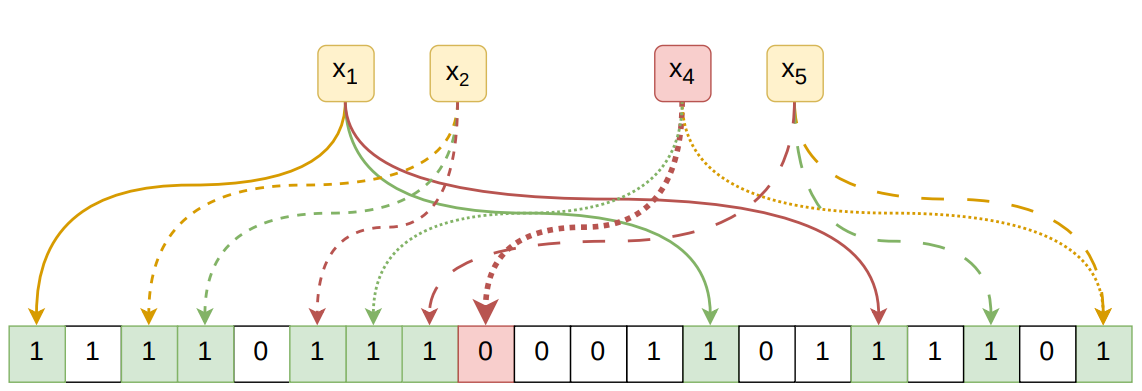
\includegraphics[width=0.5\textwidth]{img/hash/bloom.png}
    \caption{Esempio di query su Bloom Filter}
\end{figure}
\newpage
Una generalizzazione dei Bloom filter sono \textbf{Counting Bloom filter}. In queste strutture dati si tiene conto anche di quante funzioni di hash mappano in una certa posizione dato un elemento qualsiasi si verifica la presenza tramite il counting Bloom filter tramite una threshold $\theta$.

Possiamo costruire queste strutture dati andando in fase di preprocessing $\forall k \in S$ e $\forall h_i \in \mathcal{H}: [A[h_i(k)] += 1$.

In fase di query, dato $x \in \mathcal{U}$ abbiamo:
\begin{itemize}
    \item Se $\exists h_i \in \mathcal{H}$ tale che $A[h_i(x)] = 0$ o $[A[h_i(x)] \leq \theta$ allora $x \notin S$
    \item Se $\forall h_i \in \mathcal{H}$ $A[h_i(x)] > 0$ o $A[h_i(x)] > \theta$ allora "probabilmente" $x \in S$, avendo $\mathcal{P}(FP) \neq 0$
    \item $[A[h_i(x)]$ è una sovrastima del numero di elementi $x$ in $S$.
\end{itemize}
\section{Heavy Hitters Problem}
L'\textbf{heavy hitters problem} consiste nell'identificazione dell'elemento più frequente o anche detto \textbf{heavy hitter}. Questo problema non può essere risolto utilizzando un \textbf{Bloom Filter} in quanto richiederebbe troppo spazio di memorizzazione.
\begin{definizione}[\textbf{Stream di dati}]
    Con \textbf{stream di dati} si intende una sequenza di dati passati uno ad uno alla struttura dati. Quindi, data una sequenza $S = s_0,s_1, \dots ,s_{n-1}$, prima si considera $s_0$, poi $s_1 \ \dots$ fino a $s_{n-1}$ si costruisce quindi una struttura dati che può essere interrogata con nuovi valori $x \in \mathcal{U}$.
\end{definizione}

Su questa struttura dati è possibile effettuare le seguenti query:
\begin{itemize}
    \item Quante volte appare $x$ nello stream:
    \begin{equation}
        | \{ i \in \{0, 1, \dots, n - 1\}| \ s_i = x \}|
    \end{equation}
    \item Quanti elementi distinti si hanno nello stream:
    \begin{equation}
        |\{s_i | i \in \{0, 1, \dots, n - 1\}\}|
    \end{equation}
\end{itemize}
\subsection{Count–min sketch}
Una struttura dati che ci permette di risolvere questo problema è il \textbf{Count–min sketch}, la quale richiede poco spazio in memoria ed è concettualmente simile a un Bloom filter.

Questa struttura dati è definita a partire da:
\begin{itemize}
    \item Insieme universo $\mathcal{U}$.
    \item Uno stream $S$ lungo $n$ costruito da $\mathcal{U}$.
    \item Due parametri d'errore $\delta$ e $\varepsilon$. Otterremo risposte alle query "sbagliate" entro un fattore aggiuntivo $\varepsilon$ con probabilità almeno $1 - \delta$
    \item $\mathcal{H}, \ |\mathcal{H}| = l = \lceil \ln \frac{1}{\delta} \rceil$, famiglia di funzioni hash universale per $\mathcal{U}$ si impone che:
    \begin{equation}
        h_i: \mathcal{U} \to \{0, \dots, m\}, \ \forall h_i \in \mathcal{H}, \ \text{con} \ m = \left\lceil \frac{e}{\varepsilon} - 1 \right\rceil
    \end{equation}
\end{itemize}

Il \textbf{Count–min sketch} è costituito da una matrice bidimensionale $T$ con $l$ righe, una per ogni $h_i \in \mathcal{H}$, e $m$ colonne. Si hanno quindi $l$ hash table indipendenti con $m$ entry ciascuna. La matrice $T$ viene inizializzata con tutti gli elementi a $0$.

Il caricamento di $T$ avviene nel seguente modo:
\begin{itemize}
    \item Si considerano in ordine tutti gli $x_j \in S$, con $j = 0, 1, \dots, n - 1$.
    \item Sappiamo che ogni $h_i$ ha di fatto come codominio l'insieme degli indici di colonna. Quindi inserire $x_j$ in T vuol dire incrementare di 1 $T_{h_i} [h_i(x_j)]$, $\forall h_i \in H$
\end{itemize}
Queste operazioni richiedono un tempo per essere eseguite pari a $\mathcal{O}(n)$.

Su questa struttura dati è possibile eseguire la query per $q \in \mathcal{U}$ nel seguente modo:
\begin{itemize}
    \item Si applica ogni funzione di hash a $q$
    \item Si tiene traccia di ogni $T_{h_i} [h_i(q)]$, $\forall h_i \in \mathcal{H}$
    \item Si restituisce il minimo tra tali valori, che è una stima (una frequenza approssimata $\hat{a}_q$) di quante volte occorre $q$ in $S$:
    \begin{equation}
        \hat{a}_q = \min_{h_i \in \mathcal{H}} T_{h_i} [h_i(q)]
    \end{equation}
\end{itemize}
Una query si effettua in tempo $\mathcal{O}(l)$.

È possibile dimostrare che data $a_q$, ovvero la frequenza reale di $q$ in $S$, si ha che:
\begin{equation}
    a_q \leq \hat{a}_q
\end{equation} ù
Si dimostra che $a_q \leq \hat{a}_q$ a causa delle collisioni si ottengono sovrastime ma mai sottostime della frequenza.

Inoltre, è possibile dimostrare:
\begin{equation}
    \hat{a}_q \leq a_q + \varepsilon \cdot n
\end{equation}
con probabilità almeno $1 - \delta$.

Dato che la matrice bidimensionale $T$ è di dimensione $l \times m = \lceil \ln \frac{1}{\delta} \rceil \times \lceil \frac{e}{\varepsilon} \rceil$ con valori che richiedono $\log n$ bit, allora la struttura dati occupa uno spazio pari a: 
\begin{equation}
    \left( \left\lceil \ln \frac{1}{\delta} \right\rceil \cdot \left\lceil \frac{e}{\varepsilon} \right\rceil \cdot \log n \right) \ \text{bit}
\end{equation}
\begin{figure}[!ht]
     \centering
     \begin{subfigure}[b]{0.45\textwidth}
         \centering
         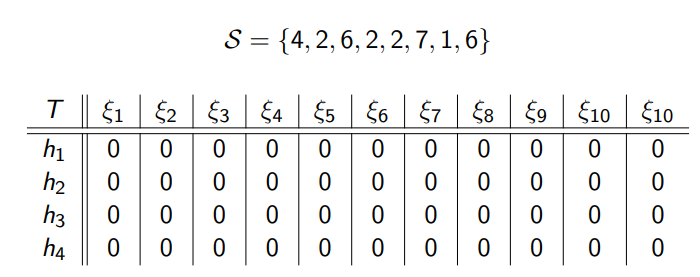
\includegraphics[width=\textwidth]{img/hash/CMS1.png}
         \caption{Inizializzazione}
     \end{subfigure}
     \hfill
     \begin{subfigure}[b]{0.45\textwidth}
         \centering
         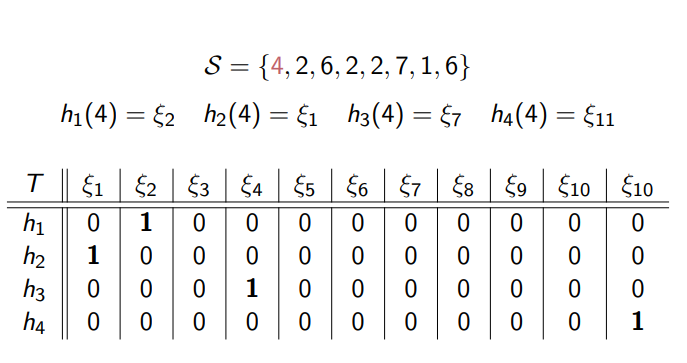
\includegraphics[width=\textwidth]{img/hash/CMS2.png}
         \caption{Inserimento del primo elemento}
     \end{subfigure}
     \hfill
     \begin{subfigure}[b]{0.45\textwidth}
         \centering
         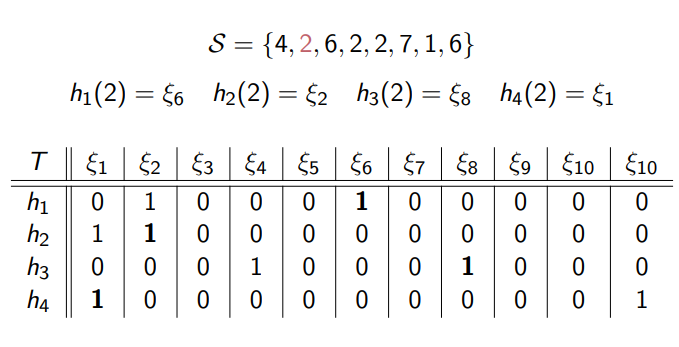
\includegraphics[width=\textwidth]{img/hash/CMS3.png}
         \caption{Inserimento del secondo elemento}
     \end{subfigure}
     \hfill
     \begin{subfigure}[b]{0.45\textwidth}
         \centering
         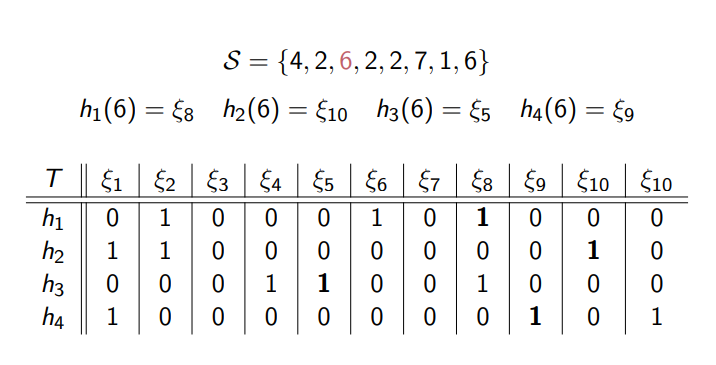
\includegraphics[width=\textwidth]{img/hash/CMS4.png}
         \caption{Inserimento del terzo elemento}
     \end{subfigure}
     \caption{Esempio di riempimento Count–min sketch}
\end{figure}
\chapter{Pattern Matching su Stringhe}
\section{Introduzione}
Il problema del Pattern Matching consiste cercare un motivo all'interno di un oggetto
più o meno complesso. In questo corso ci si concentrerà sul Pattern Matching su
Stringhe, ovvero cercare all'interno di un testo $T$ le occorrenze di un pattern $P$.
\begin{definizione}[\textbf{Stringa}]
    Definiamo una \textbf{stringa} $X$ come una giustapposizione di simboli
    appartenenti a un alfabeto $\Sigma$.
    \begin{equation}
        X=x_1x_2\dots x_n \ \ x_i \in \Sigma \ \forall i = 1, \dots, n
    \end{equation}
    In aggiunta, definiremo:
    \begin{itemize}
        \item \textbf{Stringa nulla} $\varepsilon$ è una stringa composta da 
        zero simboli.
        \item Simbolo in posizione $i$ si riferisce al simbolo in posizione 
        $i$-esima $x_i = X[i]$
        \item \textbf{Sottostringa} da $i$ a $j$ è una porzione di stringa 
        compresa tra gli indici $i$ e $j$. 
        \begin{equation}
            X[i, j] = X[i:j] = X[i]X[i+1]\dots X[j - 1]X[j]
        \end{equation}
        Posso esprimerlo attraverso la seguente notazione: $X[i, j] \lor X[i:j]$.
         Possiamo dire che una sottostringa $X[i, j]$ si definisce:
        \begin{itemize}
            \item \textbf{Propria} se $i \neq 1 \land j \neq |X|$
            \item \textbf{Impropria} altrimenti
        \end{itemize}
        \item \textbf{Prefisso} di lunghezza $j$ è una sottostringa $X[1, j]$. 
        Anche in questo caso possiamo distinguere:
        \begin{itemize}
            \item \textbf{Proprio} se $j \neq |X|$
            \item \textbf{Improprio} altrimenti
        \end{itemize}
        Per il prefisso è possibile definire anche il prefisso nullo, ovvero il 
        prefisso composto da zero caratteri ($X[1, j]=\epsilon \ \to \ j = 0$).
        \item \textbf{Suffisso} che inizia in $i$ è la sottostringa $X[i,|X|]$. 
        Di questa sottostringa posso calcolare la lunghezza del prefisso come: 
        \begin{equation}
            |X[i,|X|]| = |X| - i + 1
        \end{equation}
        Anche in questo caso possiamo distinguere:
        \begin{itemize}
            \item \textbf{Proprio} se $i \neq 1$
            \item \textbf{Improprio} altrimenti
        \end{itemize}
        È possibile definire il suffisso nullo ovvero quello composto da zero 
        caratteri ($X[i,|X|]=\epsilon \ \to \ i = |X| + 1$).
    \end{itemize}
\end{definizione}
\begin{nota}
    Una \textbf{stringa} di caratteri si differenzia da un \textbf{sequenza} 
    degli stessi caratteri dal momento che:
    \begin{itemize}
        \item \textbf{stringa}: è una giustapposizione di caratteri, quindi sono 
        tutti concatenati
        \begin{equation}
            X= \sigma_1\sigma_2\dots\sigma_n
        \end{equation}
        \item \textbf{sequenza}: è un elenco di caratteri separati da un separatore
        \begin{equation}
            X= <\sigma_1,\sigma_2,\dots,\sigma_n>
        \end{equation}
    \end{itemize}
\end{nota}

Quando si parla di string matching possiamo definire due tipi. Dati un pattern
$P$ e un testo $T$ possiamo definire lo String Matching:
\begin{enumerate}
    \item \textbf{Esatto}: consiste nel cercare le occorrenze esatte di $P$ in $T$.
    \item \textbf{Approssimato}: consiste nel cercare le occorrenze approssimate 
    di $P$ in $T$.
\end{enumerate}
\subsection{String Matching Esatto}
Possiamo definire il problema di \textbf{string matching esatto} formalmente nel seguente modo:
\begin{itemize}
    \item \textbf{input}: un testo $T$ e un pattern $P$, rispettivamente 
    $|T|=n$ e $|P|=m$, definiti su un alfabeto $\Sigma$.
    \item \textbf{output}: tutte le occorrenze esatte $i$ di $T$ ($T[i,i+m-1]=P$).
\end{itemize}
\begin{definizione}[\textbf{Occorrenza esatta}]
    Una posizione $i$ del testo $T$ tale che $T[i, i + m - 1] = P$ è 
    un'\textbf{occorrenza esatta} di $P$ in $T$.
\end{definizione}
\begin{definizione}[\textbf{Match}]
    Dati due simboli $s_1, s_2 \in \Sigma$ si ha un \textbf{match} se $s_1 = s_2$.
\end{definizione}
\begin{definizione}[\textbf{Mismatch}]
    Dati due simboli $s_1, s_2 \in \Sigma$ si ha un \textbf{mismatch} se $s_1 
    \neq s_2$.
\end{definizione}

Avendo definito il problema in questo modo è possibile definire un semplice
algoritmo che mi permette di calcolare l'output del problema. Questo algoritmo
utilizza una finestra $W$, delle stesse dimensioni del pattern, che scorre sul
testo. L'algoritmo semplice che permette di calcolare le occorrenze esatte è:
\begin{enumerate}
    \item Uso una finestra $W$ lunga $m$ che scorre lungo $T$ da sinistra a
          destra. La posizione iniziale di $W$ è $i = 1$.
    \item Si confronta ogni simbolo di $P$ con il corrispondente simbolo di $T$
          all'interno di $W$ da sinistra verso destra.
          \begin{equation}
              P[j] = T[i + j - 1] \ \forall \ j \ \text{tale che} \ 1 \leq j 
              \leq m \ \Rightarrow T[i, i + m - 1] = P
          \end{equation}
    \item $W$ viene spostata di una posizione verso destra e il confronto viene 
    ripetuto.
    \item Ultima posizione di $W$ è $i = |T| - |P| + 1 = n - m + 1$
\end{enumerate}
\begin{algorithm}
    \begin{algorithmic}
        \Function{trivial\_exact\_occurrences}{$T, P$}
        \State $n\gets |T|$
        \State $m \gets |P|$
        \State $i\gets 1$
        \While {$i \leq n - m + 1$}
        \State $j \gets 1$
        \While {$P[j] = T[i + j - 1] \ \land \ j \leq m$}
        \State $j \leq j + 1$
        \EndWhile
        \If {$j = m + 1$}
        \State $\text{output } i$
        \EndIf
        \State $i \gets i + 1$
        \EndWhile
        \EndFunction
    \end{algorithmic}
    \caption{Algoritmo banale per String Matching Esatto}
\end{algorithm}

Questo algoritmo richiede un tempo pari a $\mathcal{O}(m \cdot n)$.
\begin{nota}
    Questo algoritmo può essere migliorato spostando la finestra alla posizione 
    successiva al primo mismatch oppure si può effettuare un preprocessing del 
    pattern e del testo, permettendo di passare da una complessità quadratica ad 
    una logaritmica o lineare.
\end{nota}
\subsection{String Matching Approssimato}

Definiremo il problema di \textbf{string matching approssimato} formalmente nel seguente modo:
\begin{itemize}
    \item \textbf{input}: testo $T$ e un pattern $P$, rispettivamente $|T|=n$ e 
    $|P|=m$, definiti entrambi su un alfabeto $\Sigma$, infine, una soglia $k$ di errore. 
    \item \textbf{output}: tutte le occorrenze approssimate di $P$ in $T$ 
    respittano la soglia di errore $k$.
\end{itemize}
Introducendo una soglia di errore abbiamo bisogno di definire una metrica per 
calcolarlo. Per fare ciò si utilizza la \textit{distanza di edit} (ED) tra due 
stringhe. Tale distanza è definita come il minimo numero di operazioni di 
sostituzione, cancellazione, inserimento di un simbolo che trasformano una 
stringa nell'altra.
\begin{nota}
    \begin{equation}
        ED(X_1, X_2) \geq abs(|X_1| - |X_2|)
    \end{equation}
\end{nota}
\begin{definizione}[\textbf{Occorrenza approssimata}]
    Una posizione $i$ del testo $T$, tale che esista almeno una sottostringa 
    $S = T[i - L + 1,i]$ con $ED(P, S) \leq k$, è un'occorrenza approssimata di 
    $P$ in $T$.
\end{definizione}
\begin{nota}
    \begin{enumerate}
        \item Se $ED(P, S) \leq k$, allora $i$ è occorrenza approssimata.
        \item $ED(P, S) \geq abs(m - L) \ \Rightarrow \ $se $abs(m - L) > k$
              allora $i$ non può essere occorrenza approssimata.
    \end{enumerate}
\end{nota}
Quindi il problema formale dello \textbf{string matching approssimato} verrà definito come:
\begin{itemize}
	\item \textbf{input}: un testo $T$ e un pattern $P$, rispettivamente $|T|=n$
     e $|P|=m$, definiti entrambi su un alfabeto $\Sigma$, infine, una soglia $k$
      di errore. 
	\item \textbf{output}: tutte le occorrenze approssimate di $P$ in $T$ tale 
    che  $ED(E,S)\le k$.
\end{itemize}
Avendo definito il problema in questo modo è possibile definire un semplice 
algoritmo che mi permette di calcolare l'output del problema. Questo algoritmo
 utilizza una finestra $W$, di dimensione variabile, che scorre sul testo.
\begin{enumerate}
    \item Uso una finestra $W$ di lunghezza variabile $\in [m - k, m + k]$, per 
    un totale di $2k+1$ ampiezze da testare, che scorre lungo il testo $T$ da
     sinistra a destra. La posizione iniziale di tale finestra è $i = m - k$ e 
     la sua lunghezza iniziale è $m - k$.
    \item Se la distanza di edit tra $P$ e la sottostringa di $T$ compresa in $W$
     è $\leq \ k$, allora $i$ è occorrenza approssimata di $P$ in $T$.
    \item $W$ viene spostata a destra di una posizione.
\end{enumerate}
\begin{algorithm}
    \begin{algorithmic}
        \Function{trivial\_approx\_occurrences}{$T, P, k$}
        \State $n\gets |T|$
        \State $m \gets |P|$
        \State $i\gets m - k$
        \While {$i \leq n$}
        \State $L \gets  m - k$
        \While {$L \leq m + k \ \land \ i - L + 1 \geq 1$}
        \If {$ED(P, T[i - L + i, i]) \leq k$}
        \State $\text{output } i$
        \EndIf
        \EndWhile
        \State $i \gets i + 1$
        \EndWhile
        \EndFunction
    \end{algorithmic}
    \caption{Algoritmo banale per String Matching Approssimato}
\end{algorithm}

Questo algoritmo mi permette di calcolare il matching approssimato in tempo
$\mathcal{O}(n \cdot k \cdot m^2)$, dove $m^2$ è dovuto al calcolo della distanza
di edit tra le due sottostringhe.
\section{Ricerca esatta con Automa a Stati Finiti}
Un automa è un modello di calcolo che riconosce un linguaggio, ovvero un insieme
di stringhe che godono di una proprietà. Gli automi a stati finiti riconoscono 
un linguaggio regolare.
\begin{definizione} [\textbf{Automa a stati finiti}]
    Un Automa a Stati Finiti è formalmente una quintupla:
    \begin{equation}
        A = (Q, \Sigma, \delta, q_0, F)
    \end{equation}
    dove:
    \begin{itemize}
        \item $Q$, insieme finito di stati.
        \item $\Sigma$, alfabeto in input
        \item $\delta: Q \times \Sigma \to Q$, funzione di transizione.
              $\delta(q,\sigma)$ è lo stato di arrivo a partire da $q$ dopo la lettura
              di $\sigma$
        \item $q_0$, stato iniziale
        \item $F$ (sottoinsieme di $Q$), insieme degli stati accettanti.
    \end{itemize}
\end{definizione}
Gli automi a stati finiti possono essere rappresentati attraverso un diagramma di
stato, ovvero attraverso una struttura a grafo dove i vertici sono gli stati.
Esiste l'arco $(q_1,q_2)$ se almeno un simbolo $\sigma$ è tale per cui $\delta(q_1,\sigma) = q_2$.
L'arco $(q_1,q_2)$ viene etichettato dalla lista di simboli che permettono la
transizione da $q_1$ a $q_2$. Lo stato iniziale $q_0$ è indicato tramite un arco
entrante che non esce da uno stato, mentre gli stati accettanti sono indicati da un doppio bordo.

È possibile rappresentare la funzione di transizione $\delta$ degli automi attraverso 
una matrice $T$ con $|Q|$ righe e $|\Sigma|$ colonne. Nella generica cella 
$(q, \sigma)$ sarà contenuto il valore di $\delta(q, \sigma)$, ovvero lo stato di 
arrivo a partire dallo stato $q$ attraverso il simbolo $\sigma$.
\begin{equation}
    T[q,\sigma] = q'\iff \delta(q,\sigma) = q'
\end{equation}
\begin{definizione}[\textbf{Bordo}]
    Il \textbf{bordo} di una stringa $X$ è il più lungo prefisso \textbf{proprio} 
    di $X$ che occorre come suffisso di $X$.
\end{definizione}
\begin{esempio}
    Esempi di bordo:
    \begin{itemize}
        \item $X = baaccbbaac$ il suo bordo sarà $B(X) = baac$
        \item $X = aaaccbbaac$ il suo bordo sarà $B(X) = \varepsilon$
        \item $X = abababa$ il suo bordo sarà $B(X) = ababa$
        \item $X = aaaaaaaa$ il suo bordo sarà $B(X) = aaaaaaa$
        \item $X = a$ il suo bordo sarà $B(X) = \varepsilon$
    \end{itemize}
\end{esempio}
\begin{nota}
    Il bordo di un simbolo è sempre vuoto.
\end{nota}
\begin{definizione}[\textbf{Concatenazione}]
    La \textbf{concatenazione} di un simbolo $\sigma$ con la stringa $X$ è la
    stringa $X\sigma$.
\end{definizione}
Possiamo definire ora l'automa a stati finiti per la ricerca esatta di un pattern
$P$ di lunghezza $m$ definito su alfabeto $\Sigma$ è la quintupla $(Q, \Sigma, \delta, q_0, F)$ con:
\begin{itemize}
    \item $Q = \{0, 1, \dots, m\}$
    \item $\Sigma$ è l'alfabeto di definizione di $P$
    \item $\delta: Q \times \Sigma \to Q$ è la funzione di transizione
    \item $q_0 = 0$ è lo stato iniziale
    \item $F = \{m\}$ è lo stato accettante
\end{itemize}
A questo punto il processo di ricerca esatta attraverso un automa a stati finiti
è composto da:
\begin{enumerate}
    \item \textbf{Preprocessing del pattern}: costruisco l'automa per il pattern 
    $P$ che consiste nel calcolo della funzione di transizione $\delta$ in tempo 
    $\theta(m \cdot |\Sigma|)$.
    \item \textbf{Ricerca nel testo}: uso dell'automa per riconoscere, in un testo
     $T$ definito su alfabeto $\Sigma$, tutte le occorrenze esatte di $P$. La
      scansione del testo $T$ avviene in tempo $\theta(n)$
\end{enumerate}
\subsection{Funzione di transizione}
La funzione di transizione $\delta$ per un pattern $P$ di lunghezza $m$ definito
su un alfabeto $\Sigma$ è definita per ogni $(j, \sigma) \in Q \times \Sigma$ tale
che $\delta(j, \sigma)$ è lo stato in cui si arriva da $j$ attraverso $\sigma$:
\begin{equation}
    \delta(j, \sigma) = \begin{cases}
        j + 1 & \text{se} \ j < m \ \land \ P[j + 1] = \sigma   \\
        k     & \text{se} \ j = m \ \lor \ P[j + 1] \neq \sigma
    \end{cases}
\end{equation}
dove $k$ è la lunghezza del bordo del prefisso di $P$ di lunghezza $1, j$ a cui
è concatenato $\sigma$, ovvero:
\begin{equation}
    k = |B(P[1, j]\sigma)| \ \ k \leq j
\end{equation}

Dallo stato $0$ si arriva allo stato $0$ per qualsiasi simbolo diverso da P[1].
Dallo stato $0$ si arriva allo stato $1$ attraverso il simbolo $P[1]$. Dallo stato
$j = m$ si arriva sempre a uno stato $k \leq m$, dallo stato $m$ si può giungere
quindi di nuovo allo stato $m$.
\subsection{Scansione del testo}
La scansione del testo inizia da uno stato iniziale $j_0 = 0$. Partendo da questo
stato, leggo il simbolo in posizione $i$ del testo ($T[i]$) e mi sposto nello stato
$j_i$ attraverso la funzione di transizione $\delta(j_{i - 1}, T[i])$.
\begin{esempio}
    Consideriamo il testo $T$:
    \begin{table}[!ht]
        \centering
        \begin{tabular}{ccccccc}
            1                       & 2                      & 3                      & 4                      & 5                      & 6                      & 7                      \\ \hline
            \multicolumn{1}{|c|}{c} & \multicolumn{1}{c|}{a} & \multicolumn{1}{c|}{b} & \multicolumn{1}{c|}{a} & \multicolumn{1}{c|}{c} & \multicolumn{1}{c|}{a} & \multicolumn{1}{c|}{b} \\ \hline
        \end{tabular}
    \end{table}

    e il pattern $P$:
    \begin{table}[!ht]
        \centering
        \begin{tabular}{ccccccc}
            1                       & 2                      & 3                      & 4                      \\ \hline
            \multicolumn{1}{|c|}{a} & \multicolumn{1}{c|}{c} & \multicolumn{1}{c|}{a} & \multicolumn{1}{c|}{c} \\ \hline
        \end{tabular}
    \end{table}

    Su cui è stata definita la seguente funzione di transizione $\delta$:
    \begin{table}[!ht]
        \centering
        \begin{tabular}{|>{\columncolor[HTML]{EFEFEF}}c |c|c|c|} \hline
            $\delta$   & \cellcolor[HTML]{EFEFEF}\textbf{a} & \cellcolor[HTML]{EFEFEF}\textbf{b} & \cellcolor[HTML]{EFEFEF}\textbf{c} \\ \hline
            \textbf{0} & 1                                  & 0                                  & 0                                  \\ \hline
            \textbf{1} & 1                                  & 0                                  & 2                                  \\ \hline
            \textbf{2} & 3                                  & 0                                  & 0                                  \\ \hline
            \textbf{3} & 1                                  & 0                                  & 4                                  \\ \hline
            \textbf{4} & 3                                  & 0                                  & 0                                  \\ \hline
        \end{tabular}
    \end{table}

    La scansione del testo $T$ cercando le occorrenze esatte del pattern $P$ mi
    permette di ottenere il risultato riportato in figura \ref{fig:scansione}
    \begin{figure}[!ht]
        \centering
        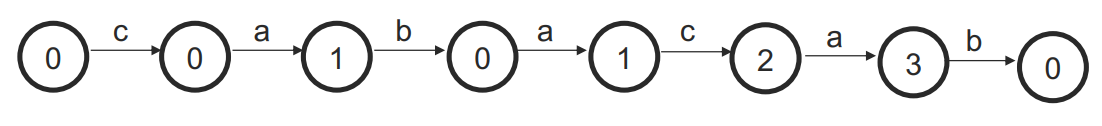
\includegraphics[width=0.5\textwidth]{img/pattern/ScansioneTesto.png}
        \caption{Risultato della scansione del testo}
        \label{fig:scansione}
    \end{figure}
\end{esempio}
A questo punto è necessario identificare un'occorrenza esatta del pattern $P$ nel
testo $T$. Per risolvere questo, partiamo dalla successione di stati che abbiamo
definito per la scansione del testo. Essa corrisponde a una successione di posizioni
su $P$, o in altre parole, a una successione di lunghezze di prefissi del pattern $P$.
\begin{teorema}
    $j_i$, con $0 \leq i \leq n$, è la lunghezza del \textbf{più lungo} prefisso
    di $P$ uguale a una sottostringa di $T$ che finisce in posizione $i$.
\end{teorema}
\begin{dimostrazione}
    È possibile dimostrare il teorema precedente con una dimostrazione per induzione:
    \begin{enumerate}
        \item \textbf{Caso base}: per lo stato $j_0 = 0$ il teorema è banalmente
              dimostrabile, in quanto il prefisso di lunghezza $0$ è il prefisso nullo
              che è sottostringa di $T$.
        \item \textbf{Passo induttivo}: se $j_{i-1}$ è la lunghezza del più lungo
              prefisso di $P$ uguale alla sottostringa di $T$ che finisce in posizione
              $i-1$, allora $j_i$ è la lunghezza del più lungo prefisso di $P$ uguale
              alla sottostringa di $T$ che finisce in posizione $i$.

              Per dimostrare il passo induttivo ci basiamo sulla seguente ipotesi:
              $j_{i-1}$ è la lunghezza del più lungo prefisso di $P$ uguale a una
              sottostringa di $T$ che finisce in posizione $i-1$.
              \begin{itemize}
                  \item \textbf{Caso 1}: $j_{i - 1} < m$ e $P[j_{i - 1} + 1] = T[i]$
                        questo implica $j_i = \delta(j_{i - 1}, T[i]) = j_{i - 1} + 1$
                        \begin{itemize}
                            \item $j_{i - 1} \neq 0$: la tesi è confermata
                            \item $j_{i - 1} = 0$ vuol dire che il carattere
                                  corrisponde con il carattere iniziale del pattern
                        \end{itemize}
                  \item \textbf{Caso 2}: $j_{i - 1} = m$ oppure
                        $P[j_{i - 1} + 1] \neq T[i]$ questo implica
                        $j_i = \delta(j_{i - 1}, T[i]) = k$ dove $k$ è la lunghezza del
                        bordo di $P[1, j_{i - 1}]T[i]$.
                        \begin{itemize}
                            \item $0 < j_{i - 1} < m$: in questo caso il valore
                                  di $k$ mi rappresenta una parte del testo per cui ho
                                  già verificato un'occorrenza esatta, questo mi viene
                                  garantito dalla definizione di bordo.
                            \item $j_{i - 1} = 0$ vuol dire che sono rimasto nello stato 0.
                            \item $j_{i - 1} = m$ ho trovato un'occorrenza esatta
                                  del pattern, inoltre per evitare di perdere delle
                                  occorrenze mi sposto in base alla lunghezza del bordo
                                  del pattern concatenato con il carattere successivo.
                        \end{itemize}
              \end{itemize}
    \end{enumerate}
\end{dimostrazione}
Questo teorema mi fornisce la garanzia che non sto perdendo delle occorrenze.
Inoltre, posso trovare la posizione di inizio dell'occorrenza esatta come $i - j + 1$.
Nel caso in cui $j_i = m$ ho identificato un'occorrenza esatta del pattern $P$.

Possiamo riassumere la scansione del testo come:
\begin{enumerate}
    \item Si parte dallo stato iniziale $0$ e si effettua una scansione di $T$
          dal primo all'ultimo simbolo.
    \item Per ogni posizione $i$ di $T$ si effettua la transizione dallo stato
          corrente $j_c$ al nuovo stato $j_f = \delta(j_c, T[i])$
    \item Ogni volta che lo stato $j_f$ è lo stato accettante ($m$), viene prodotta
          in output l'occorrenza $i - m + 1$
\end{enumerate}
\begin{algorithm}
    \begin{algorithmic}
        \Function{ASF\_exact\_occurrences}{$\delta, T, m$}
        \State $n \gets |T|$
        \State $j \gets 0$
        \For{$i \gets 1 \ \text{to} \ n$}
        \State $j \gets \delta(j, T[i])$
        \If{$j = m$}
        \State $\text{\textbf{Output}} \ i - m + 1$
        \EndIf
        \EndFor
        \EndFunction
    \end{algorithmic}
    \caption{Algoritmo per la ricerca esatta con Automa a Stati Finiti}
\end{algorithm}
Questo algoritmo viene eseguito in tempo $\theta(n)$.
\begin{esempio}
    Consideriamo il testo $T$:
    \begin{table}[!ht]
        \centering
        \begin{tabular}{ccccccccccccc}
            1                       & 2                      & 3                      & 4                      & 5                      & 6                      & 7                      & 8                      & 9                      & 10                     & 11                     & 12                     & 13                     \\ \hline
            \multicolumn{1}{|c|}{c} & \multicolumn{1}{c|}{a} & \multicolumn{1}{c|}{b} & \multicolumn{1}{c|}{a} & \multicolumn{1}{c|}{c} & \multicolumn{1}{c|}{a} & \multicolumn{1}{c|}{c} & \multicolumn{1}{c|}{b} & \multicolumn{1}{c|}{a} & \multicolumn{1}{c|}{c} & \multicolumn{1}{c|}{a} & \multicolumn{1}{c|}{b} & \multicolumn{1}{c|}{a} \\ \hline
        \end{tabular}
    \end{table}

    e il pattern $P$:
    \begin{table}[!ht]
        \centering
        \begin{tabular}{ccccccc}
            1                       & 2                      & 3                      & 4                      & 5                      & 6                      & 7                      \\ \hline
            \multicolumn{1}{|c|}{a} & \multicolumn{1}{c|}{c} & \multicolumn{1}{c|}{a} & \multicolumn{1}{c|}{c} & \multicolumn{1}{c|}{b} & \multicolumn{1}{c|}{a} & \multicolumn{1}{c|}{c} \\ \hline
        \end{tabular}
    \end{table}

    Su cui è stata definita la seguente funzione di transizione $\delta$:
    \begin{table}[!ht]
        \centering
        \begin{tabular}{|>{\columncolor[HTML]{EFEFEF}}c |c|c|c|}\hline
            $\delta$   & \cellcolor[HTML]{EFEFEF}\textbf{a} & \cellcolor[HTML]{EFEFEF}\textbf{b} & \cellcolor[HTML]{EFEFEF}\textbf{c} \\ \hline
            \textbf{0} & 1                                  & 0                                  & 0                                  \\ \hline
            \textbf{1} & 1                                  & 0                                  & 2                                  \\ \hline
            \textbf{2} & 3                                  & 0                                  & 0                                  \\ \hline
            \textbf{3} & 1                                  & 0                                  & 4                                  \\ \hline
            \textbf{4} & 3                                  & 5                                  & 0                                  \\ \hline
            \textbf{5} & 6                                  & 0                                  & 0                                  \\ \hline
            \textbf{6} & 1                                  & 0                                  & 7                                  \\ \hline
            \textbf{7} & 3                                  & 0                                  & 0                                  \\ \hline
        \end{tabular}
    \end{table}

    Otteniamo la seguente esecuzione dell'algoritmo:
    \begin{figure}[!ht]
        \centering
        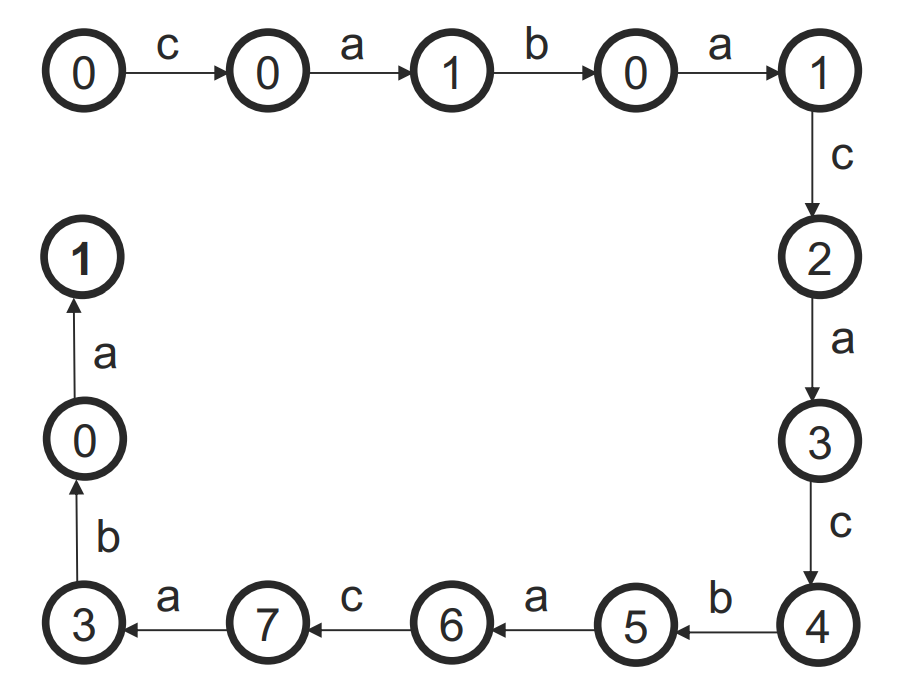
\includegraphics[width=0.3\textwidth]{img/pattern/ASF.png}
        \caption{Esecuzione dell'algoritmo per la ricerca esatta con Automa a Stati Finiti}
        \label{fig:enter-label}
    \end{figure}
\end{esempio}
\subsection{Calcolo della funzione di transizione $\delta$}
L'algoritmo più semplice che permette di calcolare i valori della funzione di
transizione $\delta$ consiste nell’applicare la funzione di transizione $\delta$ per
come è definita senza sfruttare i valori che sono già stati computati.
\begin{algorithm}
    \begin{algorithmic}
        \Function{Trivial-build-transition-function}{$P$}
        \State $m\gets |P|$
        \State $\delta \gets empty\_table (m + 1) \times | \Sigma|$
        \For{$j \gets 0 \ \text{to} \ m - 1$}
        \State $\delta(j, P[j + 1]) \gets j + 1$
        \EndFor
        \For{$j \gets 0 \ \text{to} \ m$}
        \For{$\sigma \in \Sigma$}
        \State $\delta(j, \sigma) \gets |B(P[1, j]\sigma)|$
        \EndFor
        \EndFor
        \State $\text{\textbf{return}} \ \delta$
        \EndFunction
    \end{algorithmic}
    \caption{Algoritmo banale per il calcolo della funzione di transizione $\delta$}
\end{algorithm}
Questo algoritmo richiede un tempo nel caso peggiore pari a $\mathcal{O}(m^3 | \Sigma|)$,
questo è dovuto al fatto che per calcolare il bordo è necessario un tempo, nel
caso peggiore pari a $\mathcal{O}(m^2)$.

Definiamo $\delta_j$ come la funzione di transizione di $P[1, j]$, ovvero come
una funzione:
\begin{equation}
    \delta_j: \{0, 1, \dots, j\} \times \Sigma \to \{0, 1, \dots, j\}
\end{equation}
per questa funzione possiamo definire due casi particolari:
\begin{itemize}
    \item $\delta_0$ ovvero la funzione di transizione di $P[1, 0]$ che per
          definizione è $\varepsilon$, quindi il valore di tale funzione è sempre $0$.
    \item $\delta_m$ ovvero la funzione di transizione di $P[1, m]$ la quale
          corrisponde precisamente alla funzione di transizione del pattern $P$.
\end{itemize}
Possiamo definire il calcolo della funzione di transizione $delta$ per un pattern
$P$ di lunghezza $m$ utilizzando l'induzione nel seguente modo:
\begin{itemize}
    \item Caso base: calcolo $\delta_0$
    \item Passo induttivo: calcolo $\delta_j$ da $\delta_{j - 1}$ in questo caso
          dobbiamo distinguere il caso in cui $j = 1$ e i restanti.
          \begin{itemize}
              \item Nel caso in cui $j = 1$, possiamo definire la funzione di
                    transizione come:
                    \begin{enumerate}
                        \item Prendo il valore $0$ contenuto nella cella della
                              riga $0$ di $\delta_0$ in corrispondenza del simbolo $P[1]$
                        \item Sostituisco il valore $0$ con il valore $1$ (stato
                              successivo a $0$).
                        \item Aggiungo una nuova riga (corrispondente allo stato $1$)
                        \item Copio la riga che corrisponde allo stato 0 nella riga
                              che corrisponde allo stato $1$
                        \item Rinomino $\delta_0$ in $\delta_1$
                    \end{enumerate}
              \item Mentre nel caso in cui $j \neq 1$ possiamo definire la
                    funzione di transizione come:
                    \begin{enumerate}
                        \item Prendo il valore $k$ contenuto nella cella della
                              riga $j-1$ di $\delta_{j-1}$ in corrispondenza del simbolo $P[j]$
                        \item Sostituisco il valore $k$ con il valore $j$ (stato
                              successivo a $j - 1$)
                        \item Aggiungo una nuova riga (corrispondente allo stato $j$)
                        \item Copio la riga che corrisponde allo stato $k$ nella
                              riga che corrisponde allo stato $j$
                        \item Rinomino $\delta_{j-1}$ in $\delta_j$
                    \end{enumerate}
          \end{itemize}
\end{itemize}
\begin{nota}
    Dimostrazione tramite esempi su slide.
\end{nota}
Con queste informazioni possiamo definire un algoritmo che mi permette di calcolare
la funzione di transizione $\delta$ in tempo $\theta(m \cdot |\Sigma|)$. Tale
algoritmo sfrutta le informazioni precedentemente calcolate.
\begin{algorithm}[!ht]
    \begin{algorithmic}
        \Function{Build-transition-function}{$P$}
        \State $m\gets |P|$
        \State $\delta \gets empty\_table (m + 1) \times | \Sigma|$
        \For{$\sigma \in \Sigma$}
        \State $\delta(0, \sigma) \gets 0$
        \EndFor
        \For{$j \gets 1 \ \text{to} \ m$}
        \State $k \gets \delta(j - 1, P[j])$
        \State $\delta(j - 1, P[j]) \gets j$
        \For{$\sigma \in \Sigma$}
        \State $\delta(j, \sigma) \gets \delta(k, \sigma)$
        \EndFor
        \EndFor
        \State $\text{\textbf{return}} \ \delta$
        \EndFunction
    \end{algorithmic}
    \caption{Algoritmo per il calcolo della funzione di transizione $\delta$}
\end{algorithm}
\newpage
\section{Algoritmo di Knuth-Morris-Pratt}
Questo algoritmo per la ricerca esatta è basato su un'analisi del pattern. Si hanno due fasi:
\begin{enumerate}
    \item \textbf{Preprocessing del pattern}: questa fase consiste nel calcolo
          della prefix function $\phi$, che è una funzione che associa ad ogni posizione
          del pattern la lunghezza del più lungo prefisso del pattern che è anche un
          suffisso del pattern. Questa funzione è calcolata in tempo lineare rispetto
          alla lunghezza del pattern $\mathcal{O}(m)$.
    \item \textbf{Scansione del testo}: questa fase consiste nel confrontare il
          pattern con il testo cercando di identificare le occorrenze esatte di esso.
          Questa fase è eseguita in tempo lineare rispetto alla lunghezza del testo $\mathcal{O}(n)$.
\end{enumerate}
La \textbf{prefix function} o funzione di fallimento $\phi$ è definita come segue:
\begin{equation}
    \phi: \{0, 1, \dots m\} \to \{-1, 0, \dots m\}
\end{equation}
Essa è definita come segue:
\begin{equation}
    \phi(j) = \begin{cases} |B(P[1, j])| & \text{se } 1 \leq j \leq m \\-1 & \text{se } j = 0 \end{cases}
\end{equation}

\begin{esempio}
	Calcoliamo $\phi$ sul pattern $P=abcabaabcabab$ con $m=13$.
    \begin{table}[!ht] 
        \centering
        \begin{tabular}{|>{\columncolor[HTML]{EFEFEF}}c|c|c|c|c|c|c|c|c|c|c|c|c|c|c|}\hline
            \cellcolor[HTML]{EFEFEF}\textbf{j}&\cellcolor[HTML]{EFEFEF}\textbf{0}
            &\cellcolor[HTML]{EFEFEF}\textbf{1}&\cellcolor[HTML]{EFEFEF}\textbf{2}
            &\cellcolor[HTML]{EFEFEF}\textbf{3}&\cellcolor[HTML]{EFEFEF}\textbf{4}
            &\cellcolor[HTML]{EFEFEF}\textbf{5}&\cellcolor[HTML]{EFEFEF}\textbf{6}
            &\cellcolor[HTML]{EFEFEF}\textbf{7}&\cellcolor[HTML]{EFEFEF}\textbf{8}
            &\cellcolor[HTML]{EFEFEF}\textbf{9}&\cellcolor[HTML]{EFEFEF}\textbf{10}
            &\cellcolor[HTML]{EFEFEF}\textbf{11}&\cellcolor[HTML]{EFEFEF}\textbf{12}
            &\cellcolor[HTML]{EFEFEF}\textbf{13}\\	\hline
            $\phi$& -1&0&0&0&1&2&1&1&2&3&4&5&6&2\\\hline
        \end{tabular}
    \end{table}	

\end{esempio}

Questo algoritmo è un’evoluzione dell'algoritmo banale per la ricerca delle 
occorrenze di un pattern in un testo. In particolare, l'algoritmo KMP consiste in:
\begin{enumerate}
    \item Viene usata una finestra $W$ di lunghezza $m$ che scorre sul testo $T$
          da sinistra a destra con posizione iniziale $i = 1$.
    \item Si confrontano i simboli di $P$ con i corrispondenti simboli di $T$
          all'interno della finestra $W$ andando da sinistra a destra e partendo
          dal primo simbolo di $P$.
    \item Non appena si incontra un mismatch oppure ogni simbolo di $P$ ha un
          match con il corrispondente simbolo in $W$ (i è occorrenza esatta), $W$ viene
          spostata a destra nella posizione $p = i + j - \phi(j - 1) - 1$, dove $j$ è
          l'indice del simbolo di $P$ che ha causato il mismatch, mentre $i$ è
          la posizione iniziale di $W$.
    \item L'ultima posizione di $W$ è $n - m + 1$.
\end{enumerate}
Riassumendo:
\begin{itemize}
    \item $W$ viene spostata dalla posizione $i$ alla posizione $p$, dove:
          $$p = i + j - \phi(j - 1) - 1$$ con $j$ indice del simbolo di $P$ che ha
          causato il mismatch per $W$ in posizione $i$.
    \item Il confronto riparte dal simbolo di $P$ in posizione $j = \phi(j - 1) + 1$
          e dal simbolo di $T$ in posizione $i + j - 1$.
\end{itemize}
Nel caso in cui $j = 1$, allora $p = i + 1$ e il confronto riparte dal primo
simbolo di $P$ e dal simbolo di $T$ in posizione $i + 1$.
\begin{nota}
    Chiaramente il confronto riparte dalle posizioni $i + 1$ su $T$ e $1$ su P,
    ma dire che riparte dalla posizione $i$ su $T$ e dalla posizione $0$ su $P$
    implicitamente fa riferimento ad un confronto iniziale fittizio tra $T[i]$ e
    $P[0]$ (simbolo inesistente) che di default viene considerato un match.
\end{nota}
Nel caso in cui $j = m + 1$, allora $p = i + m - \phi(m) - 1$ e il confronto
riparte dal primo simbolo di $P$ e dal simbolo di $T$ in posizione $i + m - \phi(m)$.

\begin{table}[!ht]
    \centering
    \begin{tabular}{|l|l|l|}
        \hline
                           & Automa a stati finiti       & KMP              \\ \hline
        Preprocessing di P & $\mathcal{O}(m | \Sigma |)$ & $\mathcal{O}(m)$ \\ \hline
        Scansione di T     & $\mathcal{O}(n)$            & $\mathcal{O}(n)$ \\ \hline
        Spazio             & $\mathcal{O}(m | \Sigma |)$ & $\mathcal{O}(m)$ \\ \hline
    \end{tabular}
\end{table}
Le differenze tra l'algoritmo basato sull'automa e KMP sono:
\begin{itemize}
    \item Automa:
    \begin{itemize}
        \item Efficiente per pattern piccoli, perché la memoria è contenuta 
        quindi le costanti all'interno del calcolo del tempo sono migliori.
        \item Richiede più tempo e memoria per pattern grandi, perché sprechiamo
         tempo nel calcolo del $\delta$.
        \item Ricerca di P in testi diversi utilizzando lo stesso automa
    \end{itemize}
    KMP:
    \begin{itemize}
        \item Efficiente per pattern grandi
        \item Richiede più tempo per pattern piccoli
    \end{itemize}
\end{itemize}

%% Mettere il codice solo se lo chiede
\section{Algoritmo di Baeza-Yates e Gonnet}
La ricerca esatta effettuata attraverso questo algoritmo effettua un confronto
tra i simboli del pattern e del testo in maniera non esplicita, ovvero non confronta
carattere per carattere. In questo algoritmo vengono effettuate in parallelo operazioni
bit a bit su word di bit, viene anche chiamato \textit{algoritmo bit parallel}.

Questo algoritmo segue il paradigma \textbf{shift-and} ovvero compie fondamentalmente
due sole operazioni:
\begin{itemize}
    \item \textbf{Shift} dei bit.
    \item \textbf{AND} logico tra i bit.
\end{itemize}
Come gli algoritmi visti fin ora, anche in questo caso possiamo descrivere il suo
funzionamento attraverso due fasi:
\begin{itemize}
    \item \textbf{Preprocessing del pattern} $P$ nel quale vengono calcolate 
    $|\Sigma|$ \textbf{words} ognuna di $m$ bit. Questa operazione viene eseguita 
    in tempo $\theta(|\Sigma| + m)$.
    \item \textbf{Scansione del testo} $T$ per cercare le occorrenze esatte del 
    pattern $P$. Questa operazione viene eseguita in tempo $\theta(n)$.
\end{itemize}
\subsection{Word e Operatori}
\begin{definizione}[\textbf{Word di bit}]
    Una \textbf{word di bit} è un gruppo di bit che viene trattato come un'unità
    la cui dimensione può variare e che rappresenta un valore di un certo tipo,
    come ad esempio un numero o un carattere. In una word, il bit più a destra è
    quello meno significativo, mentre quello più a sinistra è quello più significativo.
\end{definizione}
Sulle word si possono eseguire delle operazioni \textit{bit a bit}, ovvero si
esegue un'operazione tra i bit corrispondenti di due o più words di bit della
stessa lunghezza. Il valore restituito da queste operazioni è una nuova word in
cui ogni bit è il risultato dell'operazione tra i bit corrispondenti nelle word
in input. Tra queste operazioni abbiamo:
\begin{itemize}
    \item \textbf{Congiunzione logica} $\to$ AND. Questa operazione è implementata come:
          \begin{equation}
              w = w_1 \ \text{AND} \ w_2
          \end{equation}
          restituisce una word $w$ tale che:
          \begin{itemize}
              \item $w[j] = 1$ se e solo se $w_1[j] \ \text{AND} \ w_2[j] =  1$.
              \item $w[j] = 0$ altrimenti.
          \end{itemize}
    \item \textbf{Disgiunzione logica} (inclusiva) $\to$ OR. Questa operazione è 
    implementata come:
          \begin{equation}
              w = w_1 \ \text{OR} \ w_2
          \end{equation}
          restituisce una word $w$ tale che:
          \begin{itemize}
              \item $w[j] = 1$ se e solo se $w_1[j] \ \text{OR} \ w_2[j] =  1$.
              \item $w[j] = 0$ altrimenti.
          \end{itemize}
    \item \textbf{Shift dei bit} di una posizione a destra con bit più significativo a $0$
          $\to$ RSHIFT. Questa operazione è implementata come:
          \begin{equation}
              w = \text{RSHIFT}(w_1)
          \end{equation}
          restituisce una word $w$ tale che:
          \begin{itemize}
              \item $w[j] = w_1[j - 1]$ se $j \geq 2$.
              \item $w[1] = 0$ altrimenti.
          \end{itemize}
    \item \textbf{Shift dei bit} di una posizione a destra con bit più significativo a $1$
          $\to$ RSHIFT1. Questa operazione viene implementata come un RSHIFT seguito
          da un OR con una maschera in cui nella prima posizione è presente 1 e nelle altre 0.
\end{itemize}
\subsection{Preprocessing del pattern}
Dato un pattern di lunghezza $m$ e $\sigma$ in $\Sigma$, $B_{\sigma}$ è una word di $m$ bit tale che:
\begin{equation}
    B_{\sigma}[j] = 1 \iff P[j] = \sigma
\end{equation}
Viene creata una word per ogni simbolo dell'alfabeto $\Sigma$ e viene memorizzata
in una tabella $B$. Con questa rappresentazione posso effettuare le query del tipo:
"il simbolo in posizione $j$ di $P$ è uguale a un certo simbolo $\sigma$".
\begin{esempio}
	Calcoliamo la tabella $B$ per un pattern $P=abcaba$ su un alfabeto $\Sigma=\left\{a,b,c,d\right\}$.
    \begin{table}[!ht]
        \centering
        \begin{tabular}{|c|c|c|c|c|c|c|}
        \hline
            P & $a$ & $b$ & $c$ & $a$ & $b$ & $a$\\ \hline
            $B_a$ & $1$ & $0$ & $0$ & $1$ & $0$ & $1$ \\ \hline
            $B_b$ & $0$ & $1$ & $0$ & $0$ & $1$ & $0$ \\ \hline
            $B_c$ & $0$ & $0$ & $1$ & $0$ & $0$ & $0$ \\ \hline
            $B_d$ & $0$ & $0$ & $0$ & $0$ & $0$ & $0$ \\ \hline
        \end{tabular}
    \end{table}
\end{esempio}
Vediamo ora come calcolare la tabella $B$:
\begin{enumerate}
    \item tutte le word $B_{\sigma}$ vengono inizializzate a $m$ bit a $0$.
    \item viene creata una maschera $M$ di $m$ bit tutti uguali a $0$ tranne il
          più significativo che è uguale a $1$.
    \item si esegue una scansione di $P$ da sinistra a destra, e per ogni posizione
          $j$ vengono eseguite le due operazioni bit a bit:
          \begin{itemize}
              \item $B_{P[j]} = M \ \textbf{OR} \ B_{P[j]}$
              \item $M = \textbf{RSHIFT} (M)$
          \end{itemize}
\end{enumerate}
L'algoritmo per calcolare la tabella richiede un tempo pari a $\theta(|\Sigma| + m)$ ed è il seguente:
\begin{algorithm}
    \begin{algorithmic}
        \Function{Compute-table-B}{$P$}
        \State $m \gets |P|$
        \State $B \gets \text{empty table of} \ |\Sigma| \ \text{words} \ B_{\sigma}$
        \For{$\sigma \in \Sigma$}
        \State $B_{\sigma} \gets 00\dots0$
        \EndFor
        \State $M \gets 10\dots0$
        \For{$\sigma \in \Sigma$}
            \State $\sigma \gets P[j]$
            \State $B_{\sigma} \gets M \ \text{OR} \ B_{\sigma}$
            \State $M = \textbf{RSHIFT} (M)$
        \EndFor
        \State \textbf{return} $B$
        \EndFunction
    \end{algorithmic}
    \caption{Algoritmo per il calcolo della tabella $B$}
\end{algorithm}
\subsection{Scansione del testo}
La procedura per la scansione del testo è rappresentata come:
\begin{enumerate}
    \item Il testo $T$ viene scandito dalla prima all'ultima posizione.
    \item Per ogni posizione $i$ del testo $T$ viene calcolata una word $D_i$ di $m$ bit.
    \item Ogni volta che in $D_i$ il bit meno significativo è uguale a $1$, allora
          $i - m + 1$ è occorrenza esatta di $P$ in $T$.
\end{enumerate}
Dobbiamo ora definire cosa si intende con la word $D_i$. Prima di fare ciò dobbiamo
definire $P[1,j] = suff(T[1,i])$ ovvero $P[1,j]$ è uguale a un suffisso di $T[1,i]$.
\begin{definizione}[\textbf{Word $D_i$}]
    Dati $P$ lungo $m$ e $T$ lungo $n$, $D_i$ ($0 \leq i \leq n$) è una word di
    $m$ bit tale che:
    \begin{equation}
        D_i[j] = 1 \iff P[1,j] = suff(T[1,i])
    \end{equation}
    Inoltre, sappiamo per definizione che:
    \begin{itemize}
        \item $D_0 = 00\dots0$ dato che $P[1, j] \neq suff(T[1, 0]) \ \forall j$
        \item $D_i[m] = 1$ se e solo se $P[1, m] = suff(T[i-m + 1, i])$ ovvero
              si ha un’occorrenza esatta di $P$ in $T$ nella posizione $i - m + 1$.
    \end{itemize}
\end{definizione}
Ovviamente calcolare $D_i$ è sempre troppo costoso, infatti, $D_i$ viene sempre 
ottenuto a partire da $D_{i-1}$, portando a modificare l'algoritmo di scansione 
del testo nel seguente modo:
\begin{itemize}
    \item Inizia dalla word $D_0 = 00\dots0$
    \item Per ogni $i$ da $1$ a $n$ calcola la word $D_i$ a partire dalla word $D_{i-1}$.
    \item Ogni volta che $D_i$ ha il bit meno significativo uguale a $1$, viene
          prodotta in output l'occorrenza $i- m + 1$.
\end{itemize}
Vediamo ora come si calcola il valore di $D_i$ a partire da $D_{i - 1}$:
\begin{itemize}
    \item Se $j =  1$ allora posso calcolarla come:
    \begin{equation}
        D_i[1] = 1 \text{\textbf{AND}} B_{T[i]}[1]
    \end{equation}
    Perché $D_i[1] = 1\iff P[1,1] =suff(T[1,i])\iff P[1] = T[i]\iff B_{T[i]}[1]$.
    Si aggiunge $1$ per semplificare le operazioni bit a bit. 
    \item Se $J =  1$ allora posso calcolarla come:
          \begin{equation}
              D_i[j] = 1 \text{\textbf{AND}} B_{T[i]}[1]
          \end{equation}
          Si aggiunge $1$ per semplificare le operazioni bit a bit.
    \item Se $j > 1$ allora posso calcolarla come:
    \begin{equation}
        D_i[j] = D_{i - 1}[j - 1] \text{\textbf{AND}} B_{T[i]}[j]
    \end{equation}
    Perché $D_i[j] = 1 \iff P[1,j] = suff(T[1,i]) \iff P[1,j-1] = suff(T[1,i-1])
     \text{\textbf{AND}} P[j] = T[i] \iff D_{i-1}[j-1] \text{\textbf{AND}} B_{T[i]}[j]$.
\end{itemize}
In questo modo stiamo ancora aggiornando un bit alla volta, ma sfruttando le 
operazioni bit a bit si possono aggiornare tutti in tempo \textbf{costante} nel seguente modo:
\begin{equation}
    D_i = \text{\textbf{RSHIFT1}}(D_{i - 1}) \ \text{\textbf{AND}} \ B_{T[i]}
\end{equation}
Vediamo ora come implementare l'algoritmo che effettua la scansione del testo in tempo $\theta(n)$
\begin{algorithm}
    \begin{algorithmic}
        \Function{BYG}{$B, T$}
        \State $n \gets |T|$
        \State $D \gets 00\dots0$
        \State $M \gets 00\dots01$
        \For{$i \gets 1 \ \text{to} \ n$}
        \State $\sigma \gets T[i]$
        \State $D \gets \text{\textbf{RSHIFT1}}(D_{i - 1}) \ \text{\textbf{AND}} \ B_{T[i]}$
        \If{$(D \ \text{\textbf{AND}} M) = M$}
        \State \text{output} $i - m + 1$
        \EndIf
        \EndFor
        \EndFunction
    \end{algorithmic}
    \caption{Algoritmo per la scansione del testo}
\end{algorithm}

\begin{esempio}
	Siano un testo $T=babcabaadc$ e un pattern $P=abcaba$ tale che $|T| = 10$ e $|P|=6$.
     Entrambe le stringhe costruite sun un alfabeto $\Sigma=\left\{a,b,c,d\right\}$, 
	allora costruiamo la tabella $B_\sigma$: 
    \begin{table}[!ht]
        \centering
        \begin{tabular}{|c|c|c|c|c|c|c|}
        \hline
            P & $a$ & $b$ & $c$ & $a$ & $b$ & $a$\\ \hline
            $B_a$ & $1$ & $0$ & $0$ & $1$ & $0$ & $1$ \\ \hline
            $B_b$ & $0$ & $1$ & $0$ & $0$ & $1$ & $0$ \\ \hline
            $B_c$ & $0$ & $0$ & $1$ & $0$ & $0$ & $0$ \\ \hline
            $B_d$ & $0$ & $0$ & $0$ & $0$ & $0$ & $0$ \\ \hline
        \end{tabular}
    \end{table}
    I singoli passi sono i seguenti:
    \begin{itemize}
        \item Quindi partiremo da $D_0 = 000000$, leggo il primo simbolo del testo $T[1] = b$ e poi calcolo
        $$D_1=RSHIFT1(D_{0}) \text{ AND } B_b = 100000 \text{ AND } 010010 = 000000$$
        \item leggo il secondo simbolo del testo $T[2] = a$ e poi calcolo $D_2$
        $$D_2 = 100000 \text{ AND } 100101 = 100000 $$
        \item leggo il secondo simbolo del testo $T[3] = b$ e poi calcolo $D_3$
        $$D_3 = 110000 \text{ AND } 010010 = 010000 $$
        \item leggo il secondo simbolo del testo $T[4] = c$ e poi calcolo $D_4$
        $$D_4 = 101100 \text{ AND } 001000 = 001000 $$
        \item leggo il secondo simbolo del testo $T[5] = a$ e poi calcolo $D_5$
        $$D_5 = 100100 \text{ AND } 100101 = 100100 $$
        \item $\dots$
        \item leggo il secondo simbolo del testo $T[7] = a$ e poi calcolo $D_7$
        $$D_6 = 101001 \text{ AND } 100101 = 100001 $$
        \item Ho il bit LSB di $D_6$ uguale a $1$, quindi ho trovato un match che
         corrisponde a $i-m+1 =7-6+1= 2$. Poi continuo fino a quando non termino $T$.
    \end{itemize}
\end{esempio}


\section{Algoritmo di Wu e Manber}
L'algoritmo risolvere problemi di \textbf{stringmatching approssimati} e il funzionamento
è simile a \textbf{BYG}.
Riprendiamo la definizione di ricerca approssimata di un pattern $P$ in un testo $T$:
\begin{definizione}[\textbf{Occorrenza approssimata}]
    Una posizione $i$ del testo $T$ tale che esista una sottostringa $S =T[i - L + 1]$
    tale che $ED(P, S) \leq k$ è detta \textbf{occurrenza approssimata} di $P$ in $T$.
\end{definizione}

Come gli algoritmi visti fino a questo momento, quello di Wu e Manber è basato su due fasi:
\begin{enumerate}
    \item \textbf{prepocessing} del pattern $P$ nel quale vengono calcolate $|\Sigma|$
          \textbf{words} ognuna di $m$ bit. Questa operazione viene eseguita in tempo
          $\theta(|\Sigma| + m)$. (\textit{uguale a quello dell'algoritmo BYG})
    \item \textbf{Scansione del testo} $T$ per cercare le occorrenze approssimate del pattern $P$.
          Questa operazione viene eseguita in tempo $\theta(k \cdot n)$.
\end{enumerate}
\subsection{Scansione del testo}
Dato che la fase di preprocessing è equivalente a quella per l'algoritmo BYG,
passiamo subito alla scansione del testo. Per fare ciò dobbiamo definire la word
$D_i^h$, con $0 \leq h \leq k$ e $0 \leq i \leq n$.

Partiamo definiendo $P[1, j] = suff_h(T[1, i])$ ovvero $P[1, j]$ è uguale a un
suffisso di $T[1, i]$ a meno di $h$ errori. In altre parole, riesco a trovare un
suffisso $S$ di $T[1, i]$ tale che $ED(P[1, j], S) \leq h$.

Estenderemo la definizione di $D_i$ di ShiftAND al caso in cui si ammettono al più $h$ errori.
\begin{definizione}[\textbf{Word $D_i^h$}]
    Dati un pattern $P$ lungo $m$, un testo $T$ lungo $n$ e una soglia di errore $k$,
    possiamo definire la \textbf{word $D_i^h$} come una word di $m$ bit tale che:
    \begin{equation}
        D_i^h[j] = 1 \iff P[1, j] = suff_h(T[1, i])
    \end{equation}
\end{definizione}
Vediamo ora alcuni casi particolare:
\begin{itemize}
    \item $D_i^0$: ovvero la la word con $h = 0$, è per definizione la word $D_i$
          dell'algoritmo BYG.
    \item $D_0^h$: ovvero la word con $i = 0$, è tale che:
          \begin{itemize}
              \item $j \leq h \implies D_0^h[j] = 1$, questo perché $P[1, j]$ è un
                    prefisso di $T[1, 0]$ e quindi $ED(P[1, j], T[1, 0]) \leq h$.
              \item $j > h \implies D_0^h[j] = 0$, questo perché $P[1, j]$ non è un
                    prefisso di $T[1, 0]$ e quindi $ED(P[1, j], T[1, 0]) > h$.
          \end{itemize}
          Si ottiene quindi una word dove i primi $h$ bit sono uguali a $1$ e i
          restanti $m - h$ bit sono posti a $0$.
    \item $D_i^h [m] = i \iff P[1, m] = suff_h(T[1, i])$, ovvero se $P[1, m]$ è un
          suffisso di $T[1, i]$ a meno di $h$ errori, allora $D_i^h[m] = 1$. Nel
          caso particolare in cui $h = 0$ si ha un occorrenza esatta in $i - m + 1$.
          Mentre nel caso in cui $h = k$ si ha un'occorrenza approssimata in posizione $i$.
\end{itemize}
\begin{nota}
    In generale, $D_i^{h'}[j] = 1$ implica $D_i^{h}[j] = 1$ con $h > h'$. Inoltre,
    $D_{i}^{h} [j] = 1$ implica $D_{i}^{h + 1}[j + 1] = 1$ e $D_{i}^{h + 1}[j - 1] = 1$
\end{nota}
Definita la word $D_i^h$, possiamo definire la scansione del testo $T$ come una
successione di $k + 1$ scansioni, dove solamente all'iterazione $k$ si vanno a
verificare i bit finali delle word per cercare l'occorrenza approssimata.
Nello specifico, se all'iterazione $k$ si ha che $D_i^k[m] = 1$, allora si ha in
output l'occorrenza approssimata $i$.

Fino ad ora abbiamo definito come calcolare il caso in cui $h = 0$ oppure il caso
in cui $i = 0$. Vediamo ora come calcolare il caso in cui $i > 0, h > 0$.

Partiamo considerando il caso in cui $j > 1$, in questa situazione abbiamo che:
\begin{equation}
    D_i^h[j] = 1 \iff P[1, j] =suff_h(T[1, i]) \Leftarrow P[1, j - 1] = suff_h(T[1, i - 1]) \  \textbf{AND} \ T[i] = P[j]
\end{equation}
ovvero $D_i^h[j] = 1$ se e solo se $P[1, j - 1]$ è un suffisso di $T[1, i - 1]$
a meno di $h$ errori e $T[i] = P[j]$. Questo significa che $D_i^h[j] = 1$ se e solo se:
\begin{equation}
    D_{i - 1}^h[j - 1] = D_{i - 1}^h [j - 1] = 1 \ \textbf{AND} \ B_{T[i]} [j] =  1
\end{equation}
Quello appena visto non è l'unico caso, infatti possiamo avere anche:
\begin{equation}
    D_i^h[j] = 1 \iff P[1, j] =suff_h(T[1, i]) \Leftarrow P[1, j - 1] = suff_{h - 1}(T[1, i - 1])
\end{equation}
ovvero non ho ancora raggiunto il limite di errori e quindi posso ancora avere
errori senza superare la soglia $h$. Questo significa che $D_i^h[j] = 1$ se e solo se:
\begin{equation}
    D_i^h[j] = 1 \Leftarrow D_{i - 1}^{h - 1} [j - 1] = 1
\end{equation}
Un altra casistica è data dal fatto che posso avere un carattere in meno nel testo,
ottenendo quindi:
\begin{equation}
    D_i^h[j] = 1 \iff P[1, j] =suff_h(T[1, i]) \Leftarrow P[1, j] = suff_{h - 1}(T[1, i - 1])
\end{equation}
ovvero non ho ancora raggiunto il limite di errori. Questo significa che $D_i^h[j] = 1$
se e solo se:
\begin{equation}
    D_i^h[j] = 1 \Leftarrow D_{i - 1}^{h - 1} [j] = 1
\end{equation}
Il quarto e ultimo caso è dato dal fatto che posso modificare il pattern, ovvero:
\begin{equation}
    D_i^h[j] = 1 \iff P[1, j] =suff_h(T[1, i]) \Leftarrow P[1, j - 1] = suff_{h - 1}(T[1, i])
\end{equation}
ovvero non ho ancora raggiunto il limite di errori. Questo significa che $D_i^h[j] = 1$
se e solo se:
\begin{equation}
    D_i^h[j] = 1 \Leftarrow D_{i}^{h - 1} [j - 1] = 1
\end{equation}
A questo punto posso riassumere queste casistiche in un'unica formula:
\begin{equation}
    D_{i}^{h} [j] = (D_{i - 1}^{h} [j - 1] \ \textbf{AND} \ B_{T[i]} [j]) \ 
    \textbf{OR} \ D_{i - 1}^{h - 1} [j - 1] \ \textbf{OR} \ D_{i - 1}^{h - 1} [j] 
    \ \textbf{OR} \ D_{i}^{h - 1} [j - 1]
\end{equation}
Manca ora da analizzare il caso in cui $j = 1$, in questo caso se sostituiamo
$j = 1$ alla formula appena trovata otteniamo dei valori che non possiamo conoscere
(come ad esempio $D_{i -1}^h[0]$). Quindi, per risolvere questo problema, sostituiamo
questi valori con $1$, ottenendo:
\begin{equation}
    D_{i}^{h} [j] = (1 \ \textbf{AND} \ B_{T[i]} [j]) \ \textbf{OR} \ 1 \ 
    \textbf{OR} \ D_{i - 1}^{h - 1} [j] \ \textbf{OR} \ 1
\end{equation}
Definiendo la formula in questo modo possiamo sostituire tutte le operazioni che
controllano il bit in posizione $j - 1$ con l'operazione RSHIFT1, ottenendo:
\begin{equation}
    D_{i}^{h} [j] = (RSHIFT1(D_{i - 1}^{h} [j]) \ \textbf{AND} \ B_{T[i]} [j]) \
     \textbf{OR} \ RSHIFT1(D_{i - 1}^{h - 1} [j])  \ \textbf{OR} \ D_{i - 1}^{h - 1} [j] \
      \textbf{OR} \ RSHIFT1(D_{i}^{h - 1} [j])
\end{equation}
Vediamo ora come è possibile implementare l'algoritmo per la scansione del testo:
\begin{enumerate}
    \item Inizializzazione della parola $D_0^0$ a $00\dots0$.
    \item Calcolo di $D_i^0$ per $i = 1, \dots, n$, utilizzando l'algoritmo di BYG.
    \item Per $h$ da $1$ a $k$:
          \begin{enumerate}
              \item Calcolo di $D_0^h$.
              \item Per $i$ da $1$ a $n$:
                    \begin{enumerate}
                        \item Calcolo di $D_i^h$ a partire da $D_{i - 1}^h$.
                        \item Se $D_i^h[m] = 1 \ \textbf{AND} \ h = k$ allora output $i$.
                    \end{enumerate}
          \end{enumerate}
\end{enumerate}

\end{document}
